\providecommand{\main}{../../../..}
\documentclass[\main/dresen_thesis.tex]{subfiles}
\begin{document}
  \label{sec:monolayers:nanoparticle:saxs}

  By small-angle, the average size and shape of the nanoparticles is probed over a large volume of the sample.
  To evaluate the SAXS data quantitatively, a shape model is chosen for a fit to the data.
  % \begin{table}[ht]
  %   \centering
  %   \caption{\label{tab:monolayers:nanoparticle:saxs:scatteringLenghts}Core scattering length density of the three nanoparticle batches determined from the XRD and EDX analysis.}
  %   \begin{tabular}{ c | l | l | l }
  %       & \textbf{Ac-CoFe-C} & \textbf{Ac-CoFe-C-2} & \textbf{Ol-CoFe-C}\\
  %     \hline
  %     \rule{0pt}{2ex} $\rho_\mathrm{core}^\mathrm{X-ray} \, / \unit{10^{-6} \angstrom^{-2}}$     & 40.67  & 41.21 & 51.22 \\
  %     \rule{0pt}{2ex} $\rho_\mathrm{core}^\mathrm{neutron} \, / \unit{10^{-6} \angstrom^{-2}}$   & 6.198  & 6.132 & 7.082 \\
  %     \rule{0pt}{2ex} $\rho_\mathrm{shell}^\mathrm{X-Ray} \, / \unit{10^{-6} \angstrom^{-2}}$    &        &       & 41.28 \\
  %     \rule{0pt}{2ex} $\rho_\mathrm{shell}^\mathrm{neutron} \, / \unit{10^{-6} \angstrom^{-2}}$  &        &       & 5.938 \\
  %     \hline
  %   \end{tabular}
  % \end{table}

  \begin{figure}[tb]
    \centering
    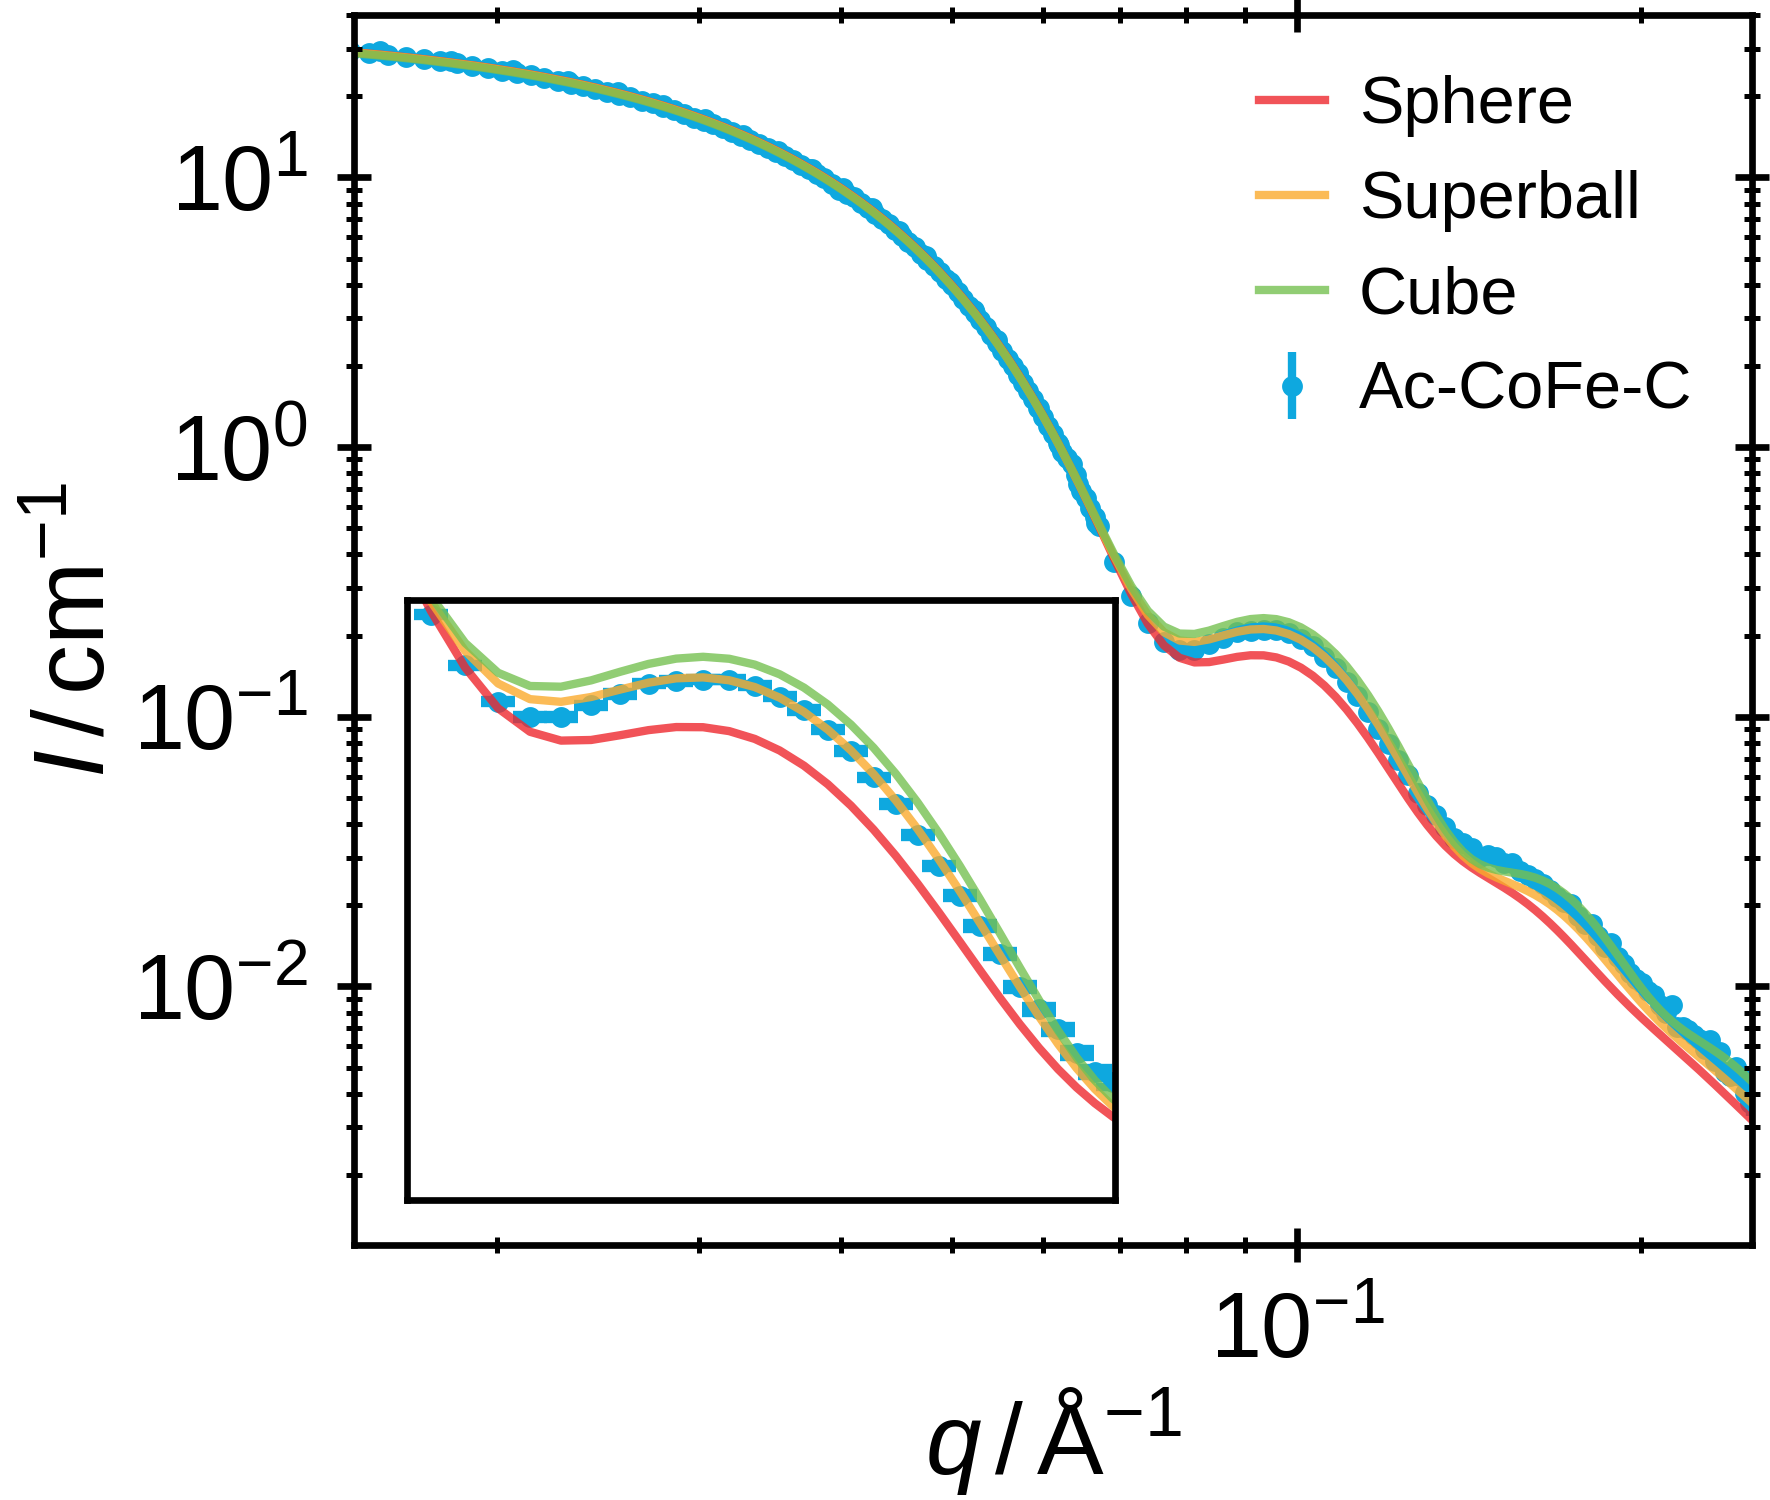
\includegraphics{monolayers_SAS_Ac_CoFe_C_ShapeModelStudy}
    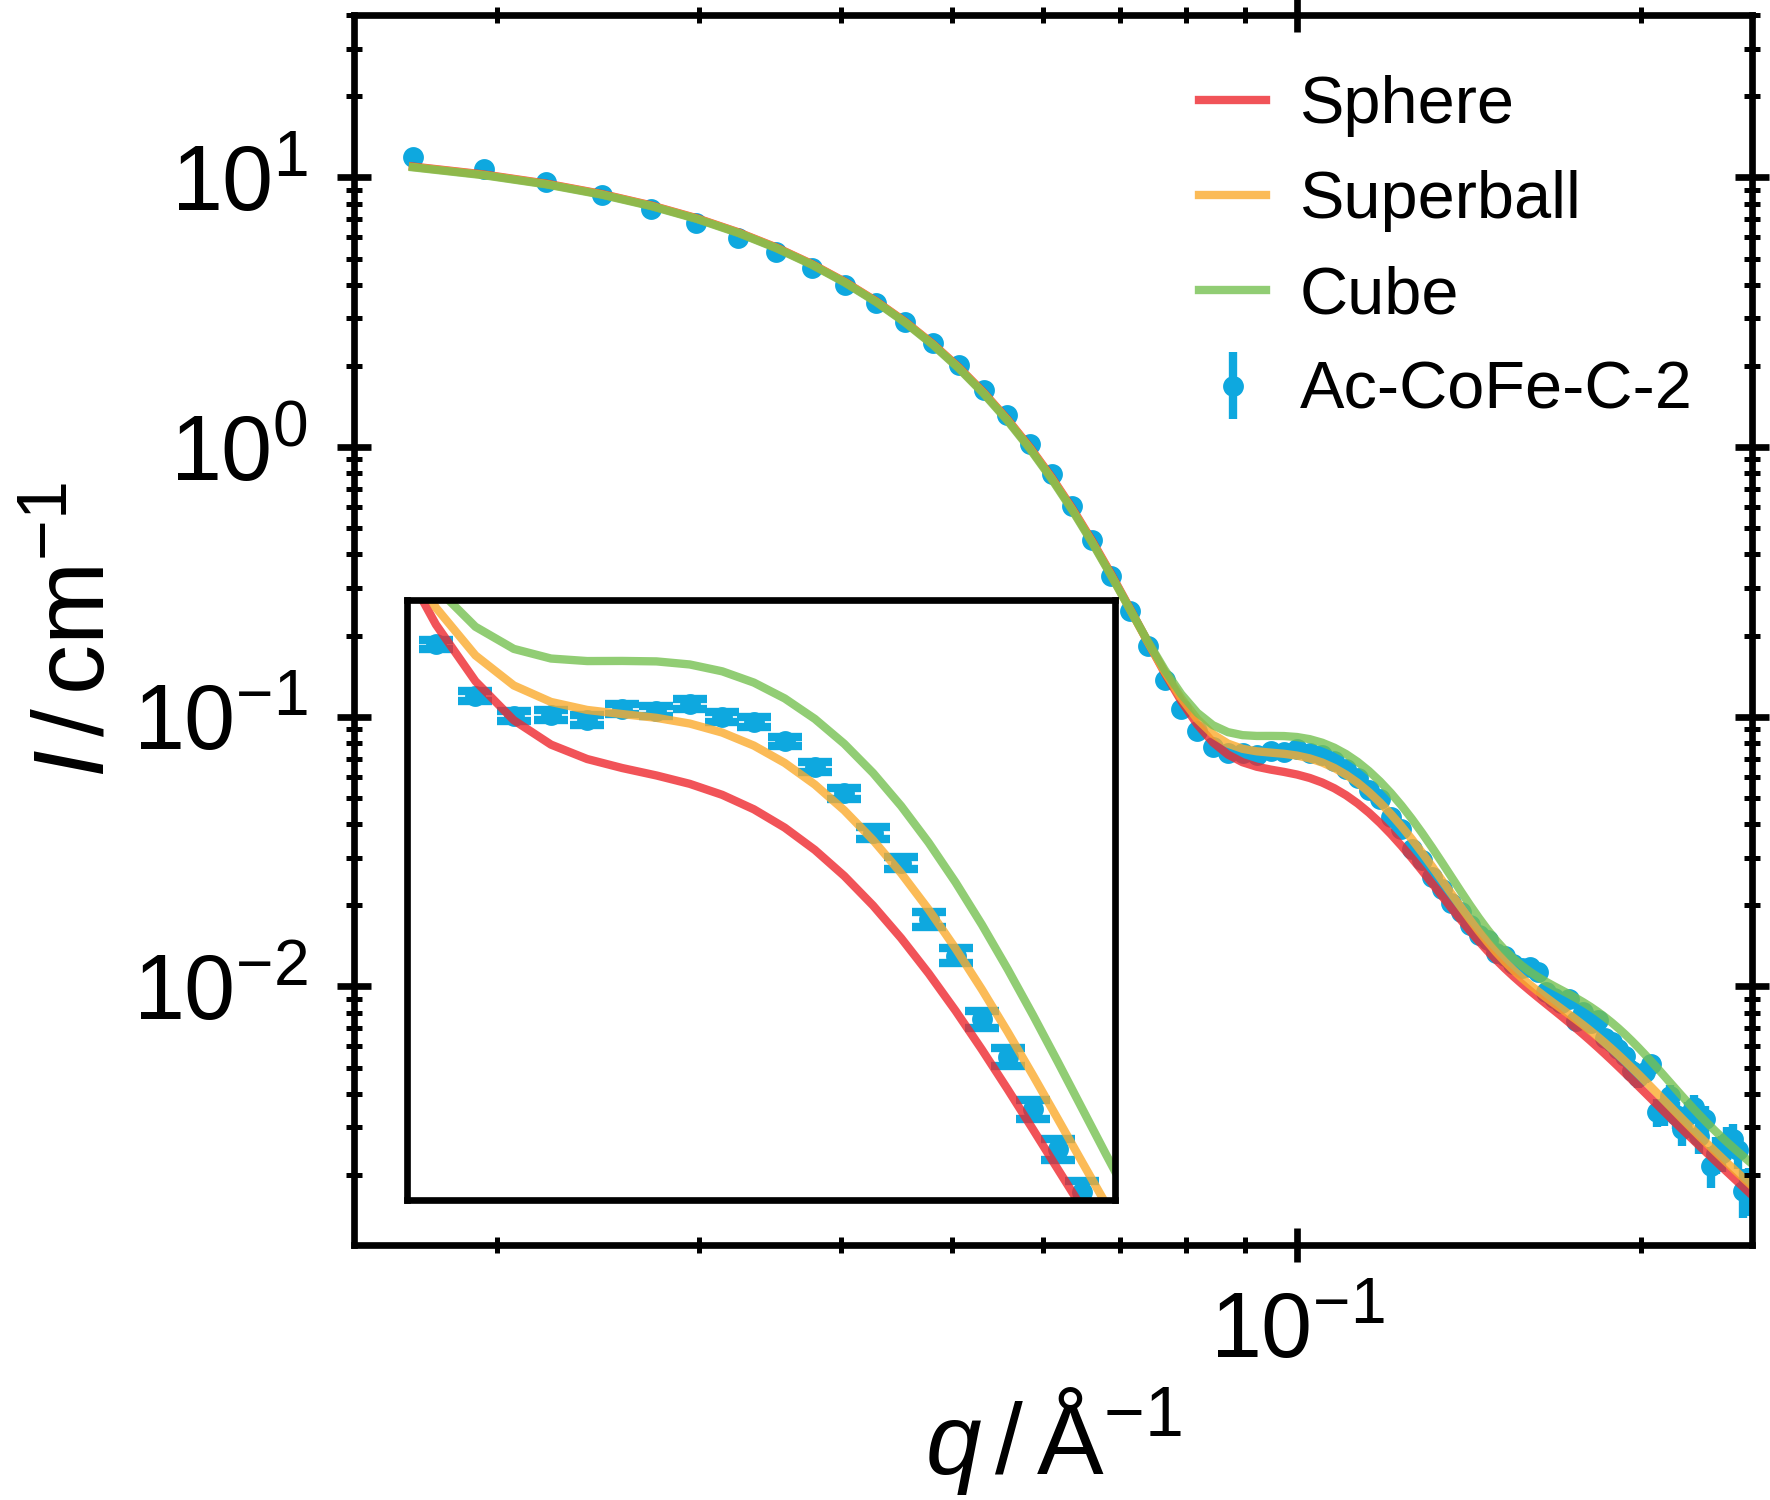
\includegraphics{monolayers_SAS_Ac_CoFe_C_2_ShapeModelStudy}
    \caption{\label{fig:monolayers:nanoparticle:sas:AcAcCoFeC}SAXS data Ac-CoFe-C (left) and Ac-CoFe-C-2 (right). In both cases the data is fit to a sphere, cube and superball form factor. The inset zooms to the first form factor maxima.}
  \end{figure}

  \paragraphNewLine{Shape Model}
    In \reffig{fig:monolayers:nanoparticle:sas:AcAcCoFeC} the SAXS data of the nanoparticles synthesized from acetylacetonates is shown.
    The data shows the first form factor minimum at a slightly smaller scattering vector for Ac-CoFe-C in direct comparison and the maxima are also qualitatively sharper for this nanoparticle batch.
    The smaller position of the minima tells that the average particle size is slightly larger for Ac-CoFe-C in comparison to Ac-CoFe-C-2, and the sharper maxima tell that Ac-CoFe-C has a smaller size distribution if both particles have a similar shape.

    To obtain a quantitative evaluation of the SAXS data, the parameters are fit to the form factors of varied shapes.
    The sphere form factor is an approximation for a small freely rotating nanoparticle that is simple to calculate and neglects the actual morphology of the particles.
    The cube form factor assumes perfectly shaped cubes with edged corners and the superball form factor allows to vary continuously in between and models a cube with rounded corners.
    Looking at the three shape model fits in \reffig{fig:monolayers:nanoparticle:sas:AcAcCoFeC}, the sphere form factor underestimates the first form factor maxima, while the cube form factor overestimates it in both cases.
    The superball form factor however is able to adjust in between and provides thereby best description of the data.

    The parameters of the three fits for both datasets are tabulated in \reftab{tab:monolayers:nanoparticle:saxs:shapeModelStudy}
    The scattering length density of the core is fixed from the results of the XRD (\refsec{sec:monolayers:nanoparticle:xrd}) and EDX (\refsec{sec:monolayers:nanoparticle:edx}) analysis of the nanoparticles.

    \begin{table}[ht]
      \centering
      \caption{\label{tab:monolayers:nanoparticle:saxs:shapeModelStudy}Parameters for the form factors of the sphere, cube and superball shown in \reffig{fig:monolayers:nanoparticle:sas:AcAcCoFeC}. 
      The size of the sphere and superball are given in terms of the radius $R$, the size of the cube is given in terms of the edge length $a$.
      The respective log-normal size distribution $\sigma_R$ and $\sigma_a$. $n$ is the particle density in dispersion, $p$ the superball exponent and $\rho_\mathrm{core}$, $\rho_\mathrm{solvent}$ the scattering length densities of the particle and the solvent respectively. From the fitted results, the mass concentration $c_m$ is given.}
      \begin{tabular}{ c | l | l | l }
        \textbf{SAXS}  & \textbf{Sphere} & \textbf{Cube} & \textbf{Superball}\\
        \hline
          \multicolumn{4}{l}{\textbf{Ac-CoFe-C}}\\
        \hline
        \rule{0pt}{2ex} $R, \, a \, / \unit{nm}$                      & $5.56(2)$      & $9.01(2)$  & $4.69(1)$\\
        \rule{0pt}{2ex} $\sigma_R, \, \sigma_a \, / \unit{\%}$        & $13.0(3)$      & $10.7(2)$  & $11.9(1)$\\
        \rule{0pt}{2ex} $n \, / 10^{-8} \angstrom^{-3}$               & $0.0425(4)$    & $0.0456(3)$& $0.0439(2)$\\
        \rule{0pt}{2ex} $p$                                           & $1$            & $\infty$   & $2.66(9)$\\
        \hline
        \rule{0pt}{2ex} $\rho_\mathrm{core}    \, / \unit{10^{-6} \angstrom^{-2}}$     & \multicolumn{3}{c}{40.67}\\
        \rule{0pt}{2ex} $\rho_\mathrm{solvent} \, / \unit{10^{-6} \angstrom^{-2}}$     & \multicolumn{3}{c}{6.46}\\
        \hline
        \rule{0pt}{2ex} $c_m \, / \unit{mg\, mL^{-1}}$                & $1.56(2)$      & $1.70(2)$  & $1.63(2)$\\
        \hline
        \rule{0pt}{2ex} $\chi^2$                                      & $168.7$        & $69.7$     & $17.8$\\
        \hline
        \hline
        \multicolumn{4}{l}{\textbf{Ac-CoFe-C-2}}\\
        \hline
        \rule{0pt}{2ex} $R, \, a \, / \unit{nm}$                      & $4.98(2)$      & $8.10(4)$  & $4.29(4)$\\
        \rule{0pt}{2ex} $\sigma_R \, / \unit{\%}$                     & $15.9(4)$      & $13.6(4)$  & $15.0(4)$\\
        \rule{0pt}{2ex} $n \, / 10^{-8} \angstrom^{-3}$               & $0.0287(3)$    & $0.0307(4)$& $0.0293(3)$\\
        \rule{0pt}{2ex} $p$                                           & $1$            & $\infty$   & $2.16(2)$\\
        \hline
        \rule{0pt}{2ex} $\rho_\mathrm{core}    \, / \unit{10^{-6} \angstrom^{-2}}$     & \multicolumn{3}{c}{41.21}\\
        \rule{0pt}{2ex} $\rho_\mathrm{solvent} \, / \unit{10^{-6} \angstrom^{-2}}$     & \multicolumn{3}{c}{8.01}\\
        \hline
        \rule{0pt}{2ex} $c_m \, / \unit{mg\, mL^{-1}}$                & $0.77(1)$      & $0.84(2)$  & $0.80(2)$\\
        \hline
        \rule{0pt}{2ex} $\chi^2$                                      & $69.4$         & $70.8$     & $51.9$\\
        \hline
        \hline
        \multicolumn{4}{l}{\textbf{Ol-CoFe-C}}\\
        \hline
        \rule{0pt}{2ex} $r_\mathrm{core}, a_\mathrm{core} \, / \unit{nm}$    & $6.02(7)$     & $6.06(10)$   & $5.17(5)$\\
        \rule{0pt}{2ex} $d_\mathrm{shell} \, / \unit{nm}$                    & $0.30(1)$     & $2.20(7)$    & $0.59(4)$\\
        \rule{0pt}{2ex} $\sigma_R , \, \sigma_a / \unit{\%}$                 & $8.9(1)$      & $3.7(4)$     & $8.3(1)$\\
        \rule{0pt}{2ex} $n \, / 10^{-8} \angstrom^{-3}$                      & $0.0181(1)$   & $0.0251(3)$  & $0.0186(1)$\\
        \rule{0pt}{2ex} $p$                                                  & $1$           & $\infty$     & $1.50(5)$\\
        \hline
        \rule{0pt}{2ex} $\rho_\mathrm{core}    \, / \unit{10^{-6} \angstrom^{-2}}$     & \multicolumn{3}{c}{51.22}\\
        \rule{0pt}{2ex} $\rho_\mathrm{shell}    \, / \unit{10^{-6} \angstrom^{-2}}$    & \multicolumn{3}{c}{41.28}\\
        \rule{0pt}{2ex} $\rho_\mathrm{solvent} \, / \unit{10^{-6} \angstrom^{-2}}$     & \multicolumn{3}{c}{8.01}\\
        \hline
        \rule{0pt}{2ex} $c_m \, / \unit{mg\, mL^{-1}}$                & $1.23(4)$      & $0.91(5)$  & $0.94(3)$\\
        \hline
        \rule{0pt}{2ex} $\chi^2$                            & $47.2$        & $69.4$       & $34.3$\\
        \hline
      \end{tabular}
    \end{table}

  \paragraphNewLine{Core-Shell Form Factor for Ol-CoFe-C}
    \begin{figure}[tb]
      \centering
      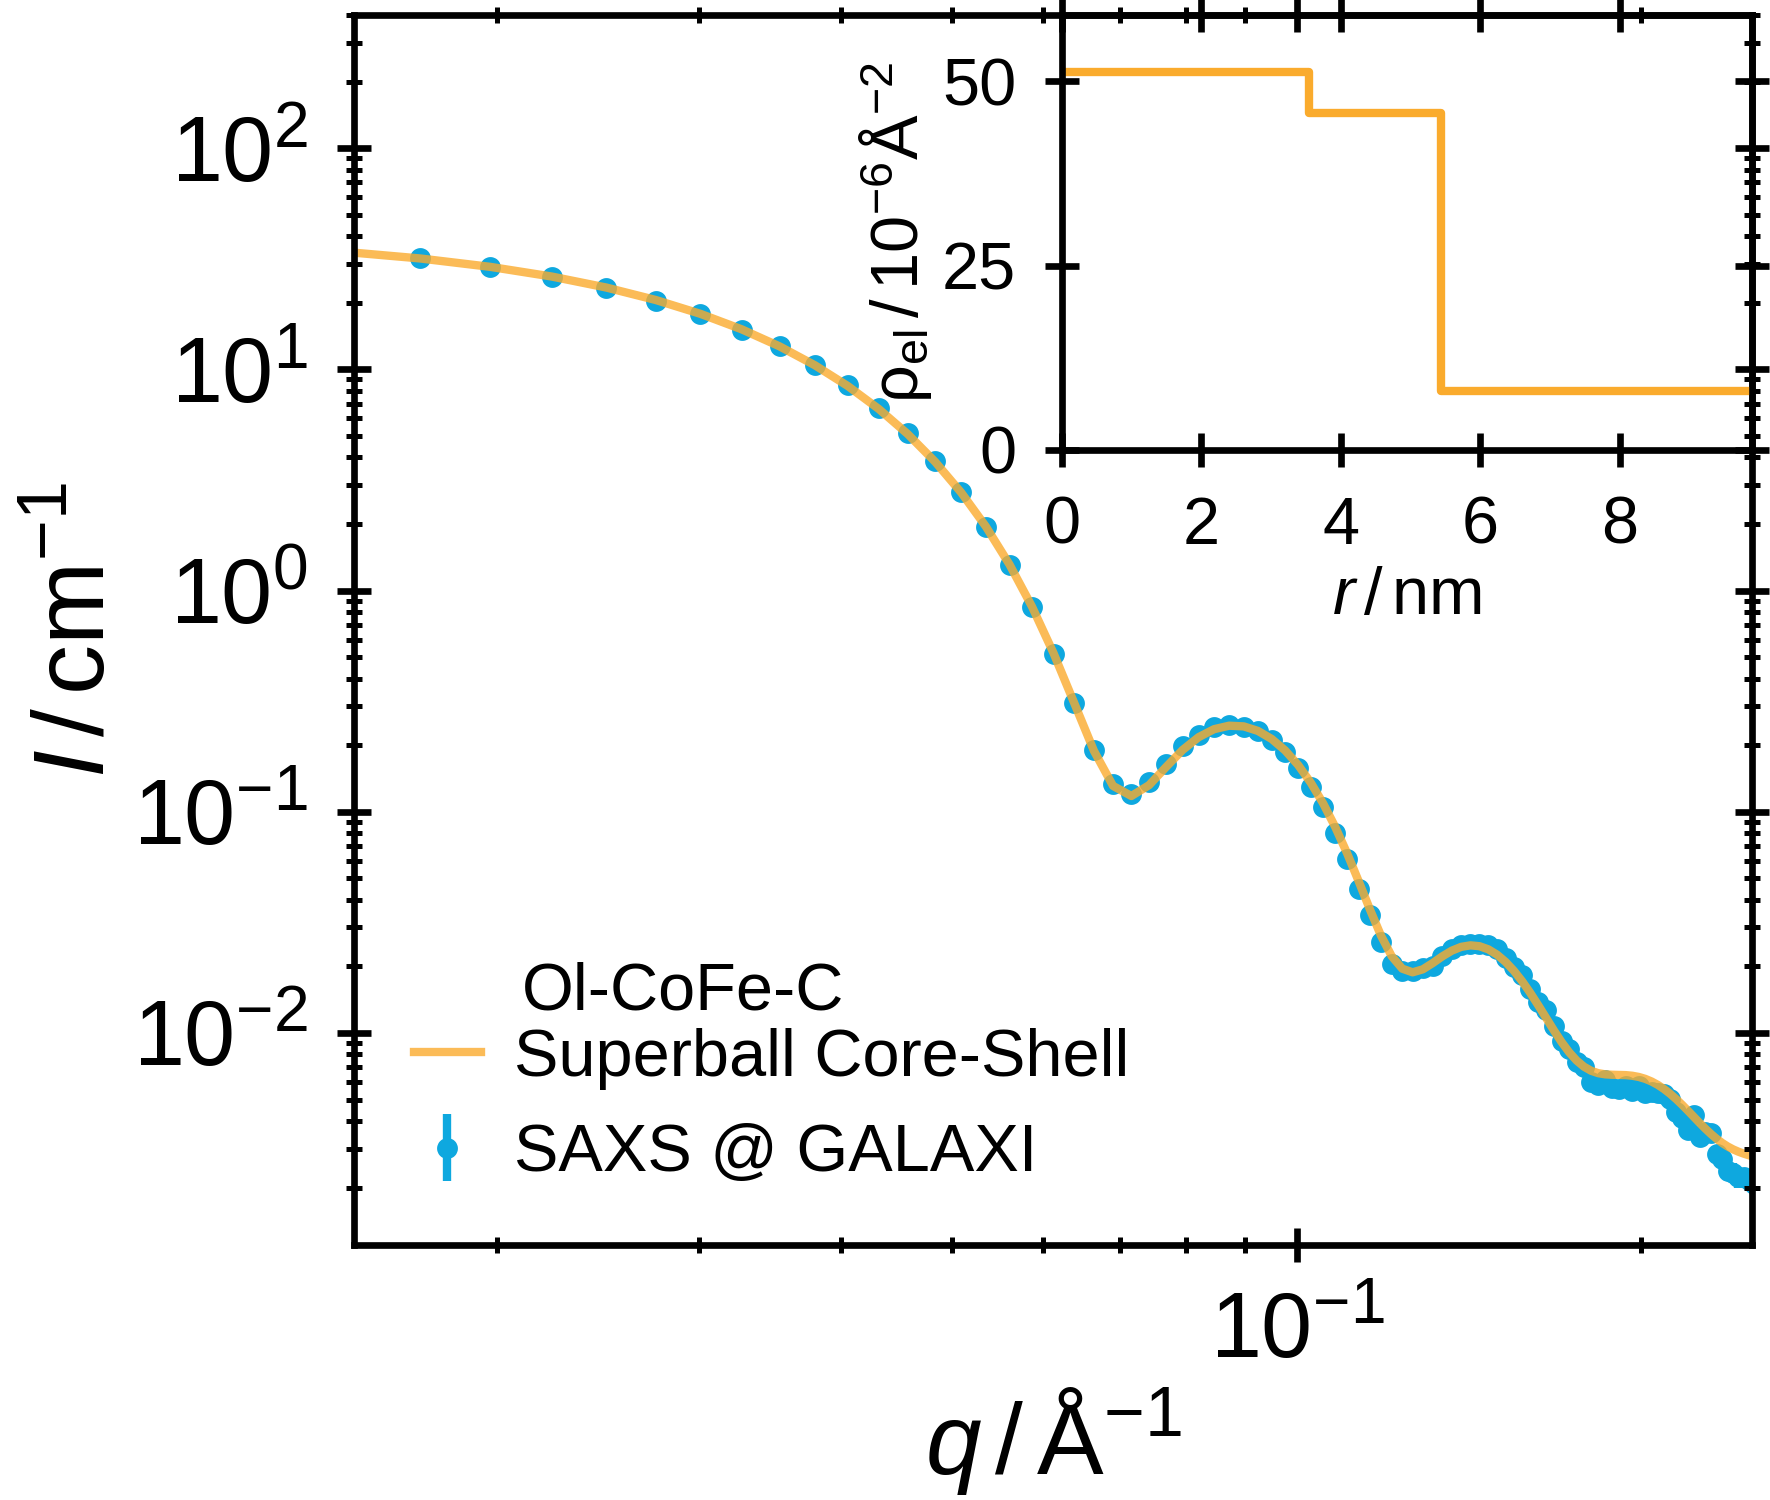
\includegraphics{monolayers_SAS_Ol_CoFe_C_ShapeModelStudy}
      \caption{\label{fig:monolayers:nanoparticle:sas:OlCoFeC}SAXS data Ol-CoFe-C, where the data is fit to a sphere, cube and superball form factor. Additionally a zoom to the first form factor maxima and two minima around it is shown in the inset.}
    \end{figure}
    To evaluate the SAXS data of the oleate nanoparticles, the form factors are further extended to allow for a variable core-shell structure.
    \reffig{fig:monolayers:nanoparticle:sas:OlCoFeC} shows the experimental data and the best fits obtained for the three core-shell shapes.
    The measured form factor presents better defined minima than the acetylacetonates nanoparticles and the third form factor maxima is recognizable, which is a sign for the smaller size-distribution.
    Comparing the best fits of the form factors for the three shapes, the contrast between them is even more apparent in this nanoparticle batch.
    While the spherical form factor is unable to catch the second form factor maxima properly, the cube form factor needs to assume a too small size distribution if it wants to catch the first form factor maxima properly.
    The superball form factor provides a solution that is in between and provides thereby an intensity profile that is closer to the measured data.
    The parameters of the three models are tabulated in \reftab{tab:monolayers:nanoparticle:saxs:shapeModelStudy}.

    As for the case of the acetylacetonates, SLD of the core is fixed from the results of the XRD (\refsec{sec:monolayers:nanoparticle:xrd}) and EDX (\refsec{sec:monolayers:nanoparticle:edx}), with a w\"ustite core and cobalt ferrite shell.
    The fitted size distribution is a log-normal distribution for the complete particle size $R \eq r_\mathrm{core} + d_\mathrm{shell}$ instead of only the core or shell, which is comparable to size distributions measured from TEM.
    
  \paragraphNewLine{Comparison of SAXS with TEM and XRD}
    To compare the sizes by the best superball fits obtained with SAXS to the sizes determined by TEM and XRD, they are listed in \reftab{tab:monolayers:nanoparticle:saxs:sizeComparison}.
    For Ac-CoFe-C and Ol-CoFe-C, the sizes obtained from SAXS and TEM are in a similar order of magnitude and deviate less than $10 \%$ from each other.
    For Ac-CoFe-C-2 the deviation is larger and especially the obtained size distribution is of greater magnitude in SAXS in contrast to TEM.
    Possibly, the evaluated TEM micrographs covered a too small specimen size and therefore the obtained size and size distribution don't reflect the true averaged sizes of the nanoparticle batch.

    The comparison with XRD, shows that for both cases of Ac-CoFe-C, the obtained crystallite sizes are smaller than the SAXS results.
    This hints to lattice disorder in the nanoparticle volume, which results in broadened peaks and therefore the smaller XRD values.

    \begin{table}[ht]
      \centering
      \caption{\label{tab:monolayers:nanoparticle:saxs:sizeComparison}Comparison of sizes.}
      \begin{tabular}{ c | l | l | l }
                            & \textbf{SAXS} & \textbf{TEM} & \textbf{XRD}\\
        \hline
        \multicolumn{4}{l}{\textbf{Ac-CoFe-C}}\\
        \hline
        $a \, / \unit{nm}$  & $9.38(2)$       & $10.1(1)$ & $5.285(3)$\\
        $\sigma_a \, / \%$  & $11.9(1)$       & $13.9(9)$ & \\
        \hline
        \multicolumn{4}{l}{\textbf{Ac-CoFe-C-2}}\\
        \hline
        $a \, / \unit{nm}$  & $8.58(8)$       & $10.8(1)$ & $5.916(5)$\\
        $\sigma_a \, / \%$  & $15.0(4)$       & $9.9(8)$  & \\
        \hline
        \multicolumn{4}{l}{\textbf{Ol-CoFe-C}}\\
        \hline
        $a_\mathrm{core} \, / \unit{nm}$      & $10.3(1)$       &           & $9.767(3)$\\
        $d_\mathrm{shell} \, / \unit{nm}$     & $0.6(4)$        &           & $3.124(1)$\\
        $a_\mathrm{total} \, / \unit{nm}$     & $11.5(4)$       & $10.9(1)$ & $12.891(3)$\\
        $\sigma_a \, / \%$                    & $8.3(1)$        & $8.8(3)$  & \\
        \hline
      \end{tabular}
    \end{table}
  % From TEM, a first estimate of the particle size ($10.1 \unit{nm}$) and size distribution ($13.9 \%$) is given.


  %   The comparison between the Ol-CoFe-C and Ac-CoFe-C small-angle scattering data shows on a qualitative level that the nanocubes synthesized following the oleate route have a smaller size distribution and higher homogeneous sample quality as more oscillations are visible with more pronounced minima, confirming the result observed from TEM.
  %   However, it also shows that Ol-CoFe-C is only weakly magnetic whereas the particles in Ac-CoFe-C have a stronger magnetic moment, which is visible in the greater splitting of $I(+)$ and $I(-)$ in SANSPOL.

  %   \begin{figure}[tb]
  %     \centering
  %     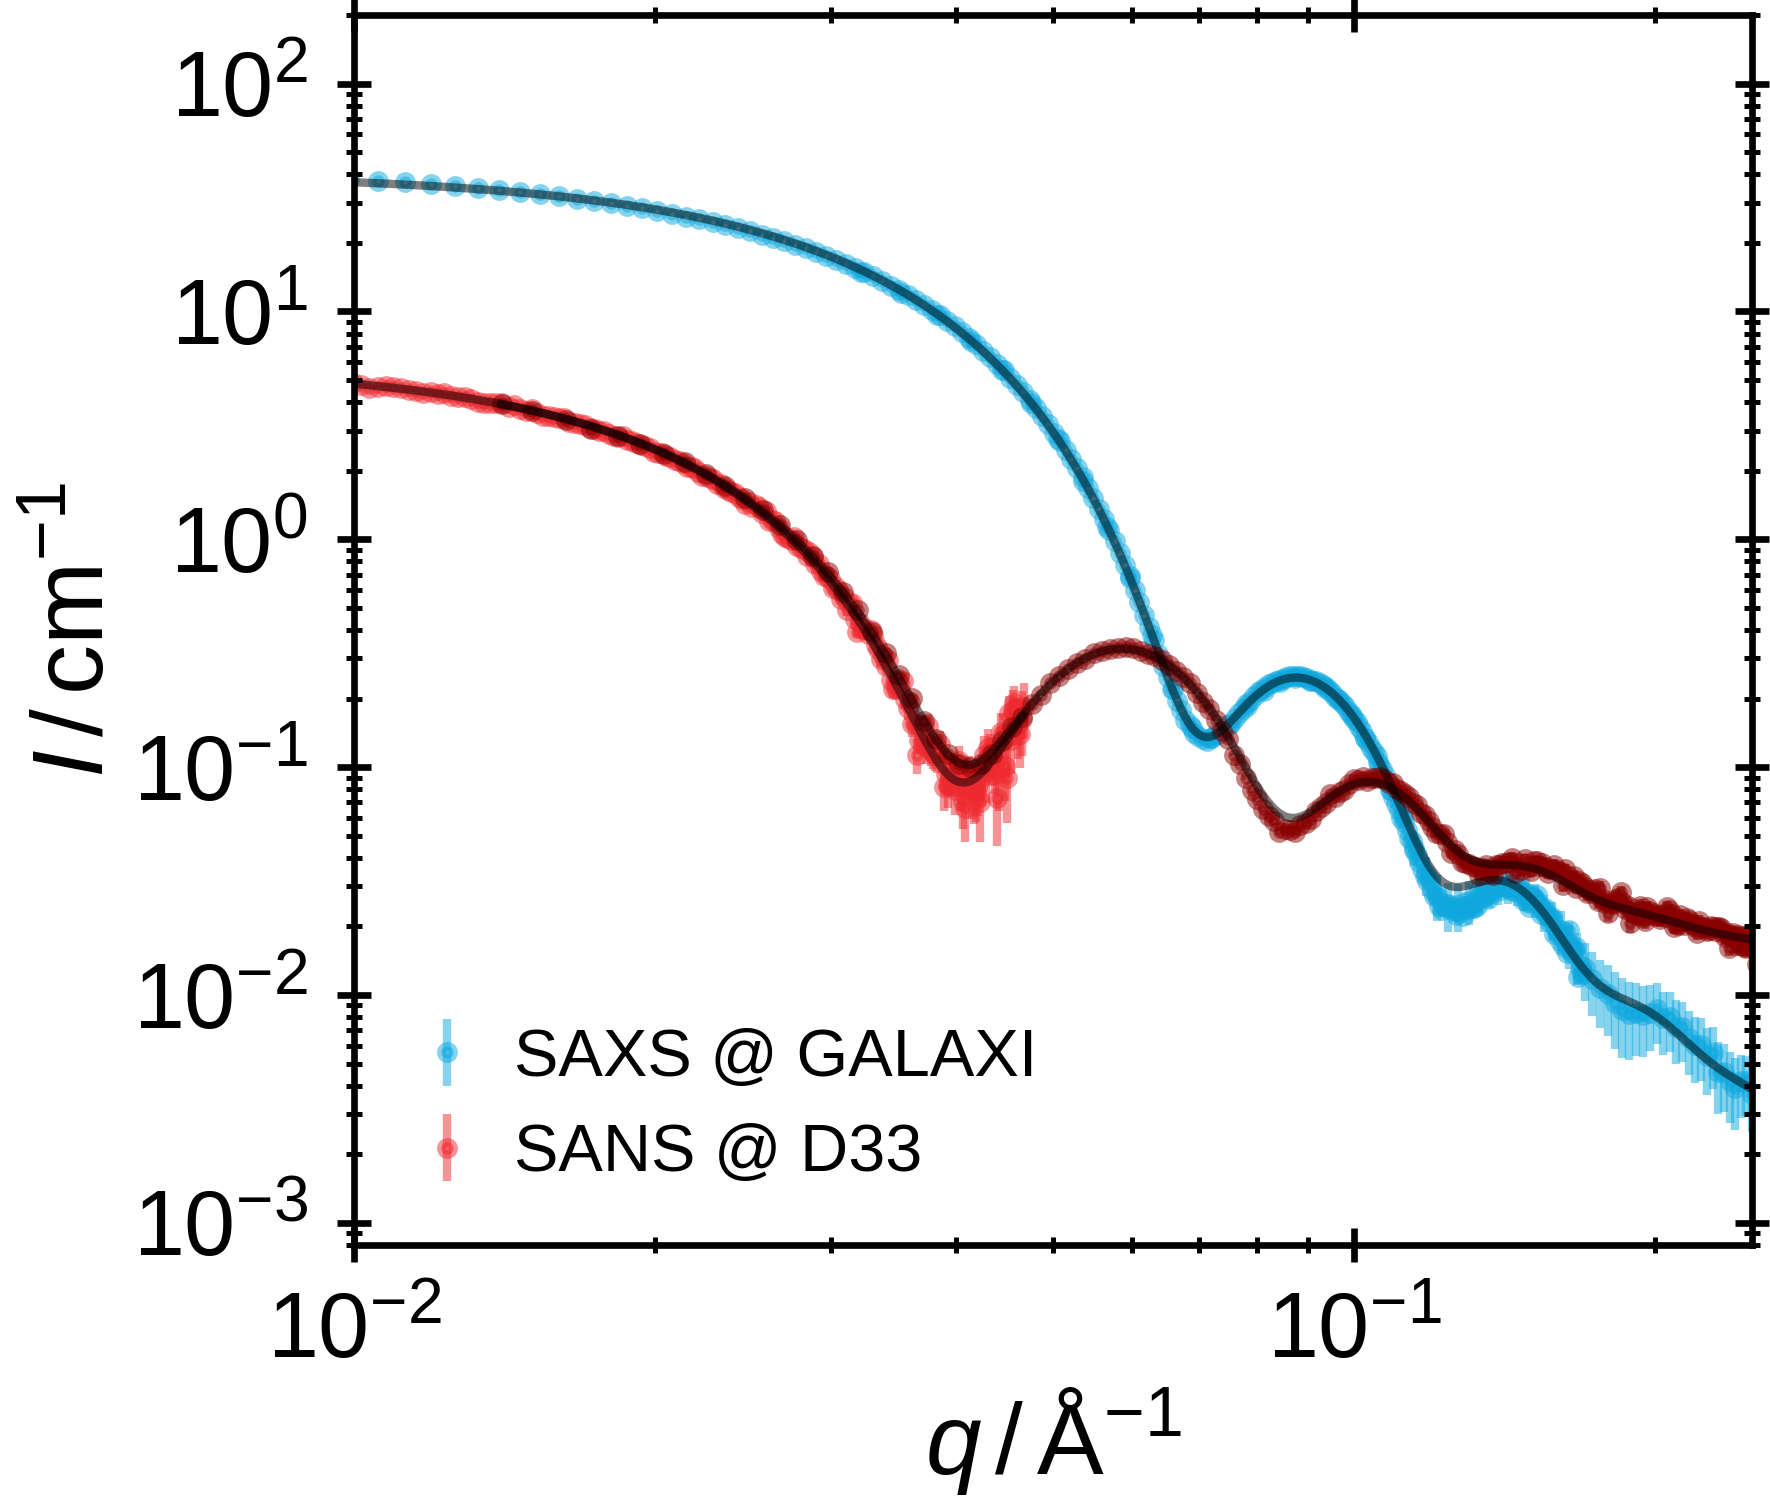
\includegraphics{monolayers_SAS_Ol_CoFe_C_SASFit}
  %     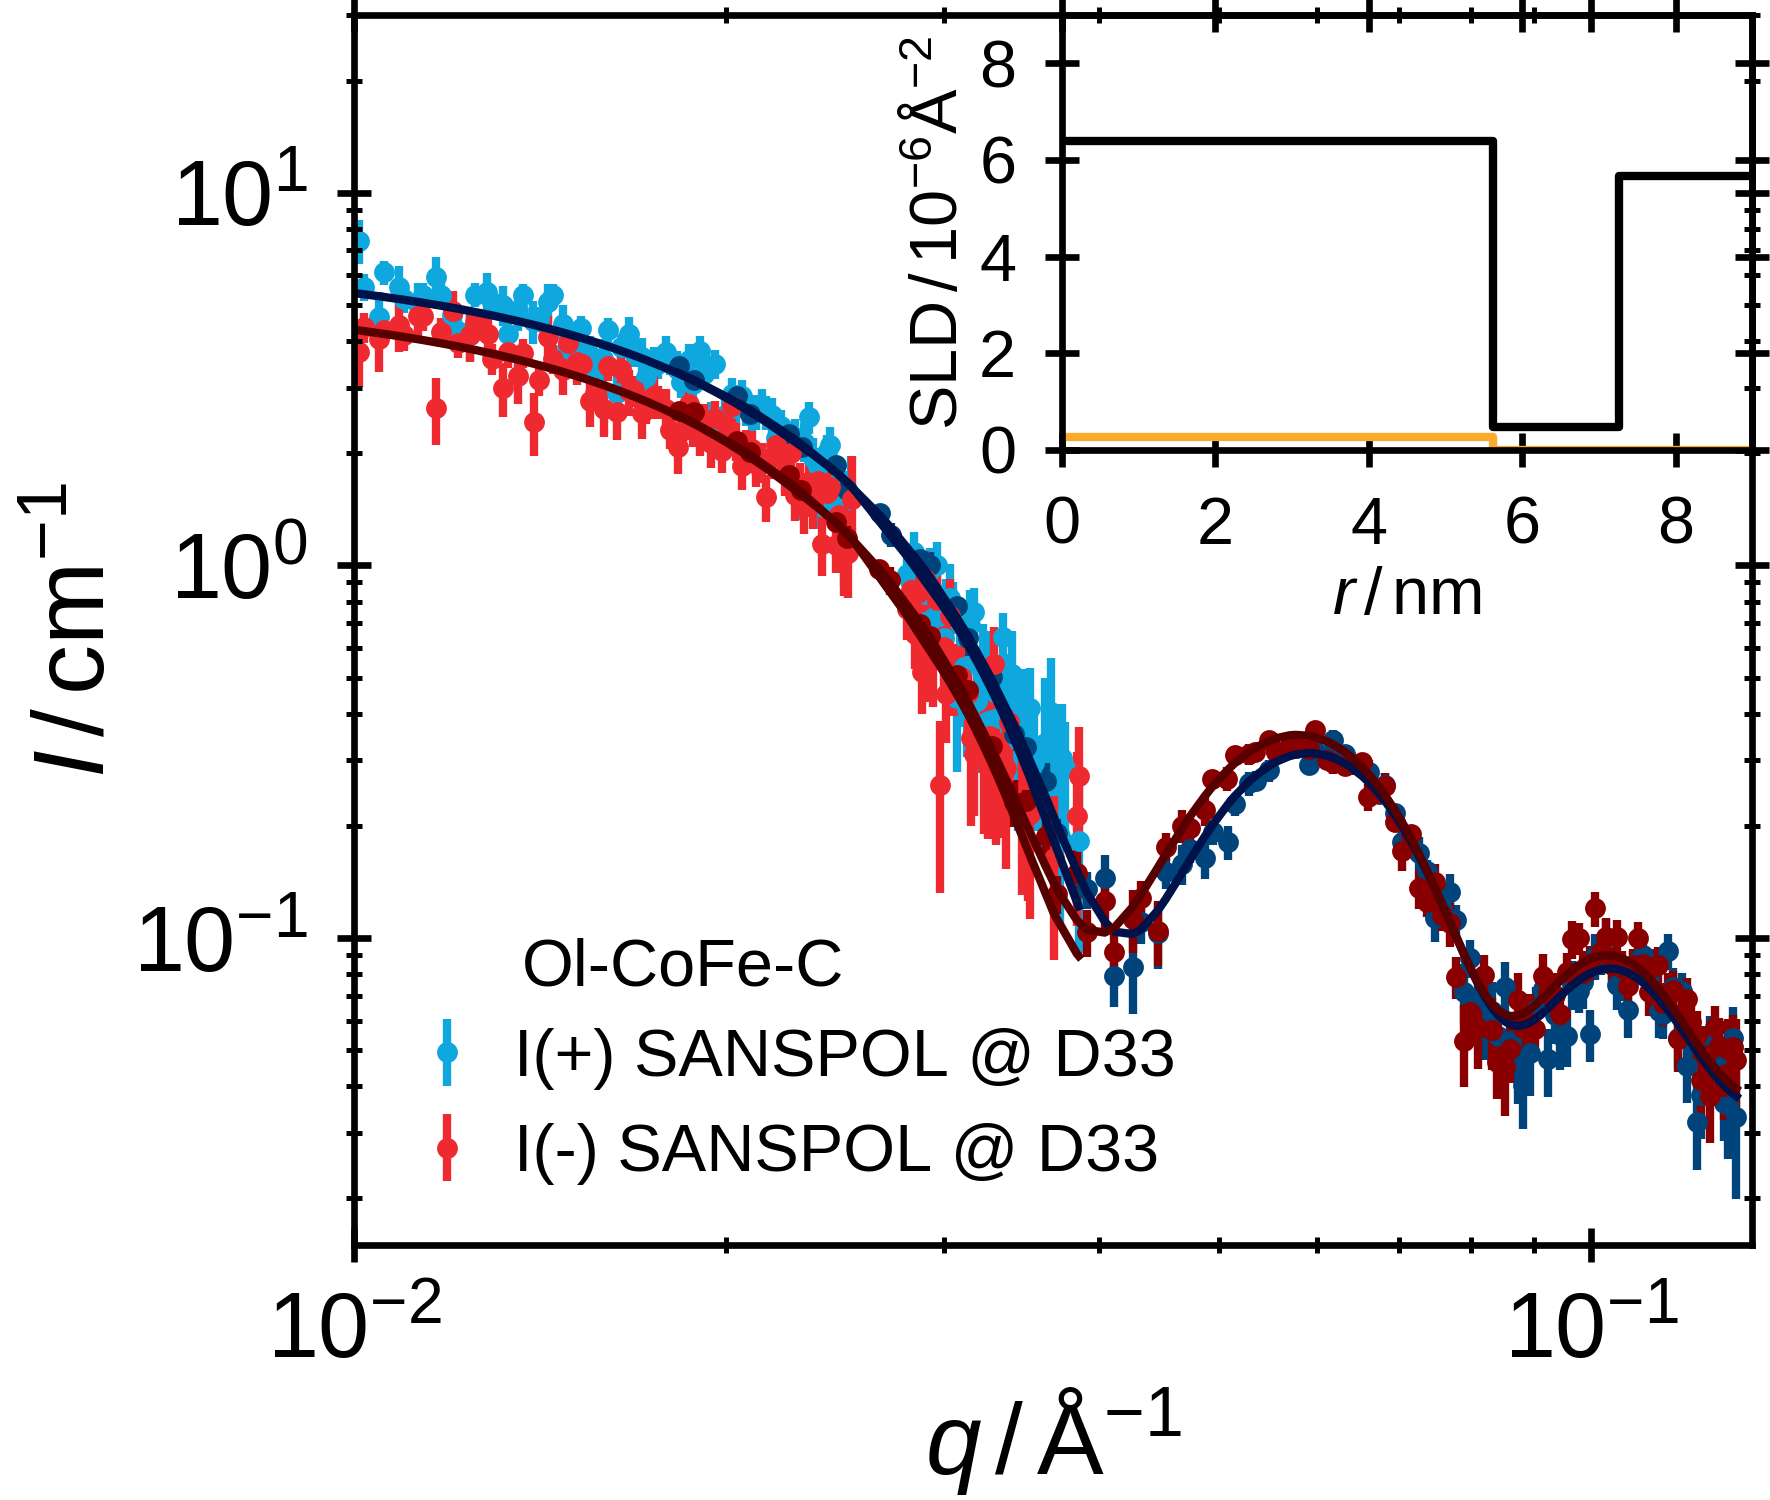
\includegraphics{monolayers_SAS_Ol_CoFe_C_SANSPOLFit}
  %     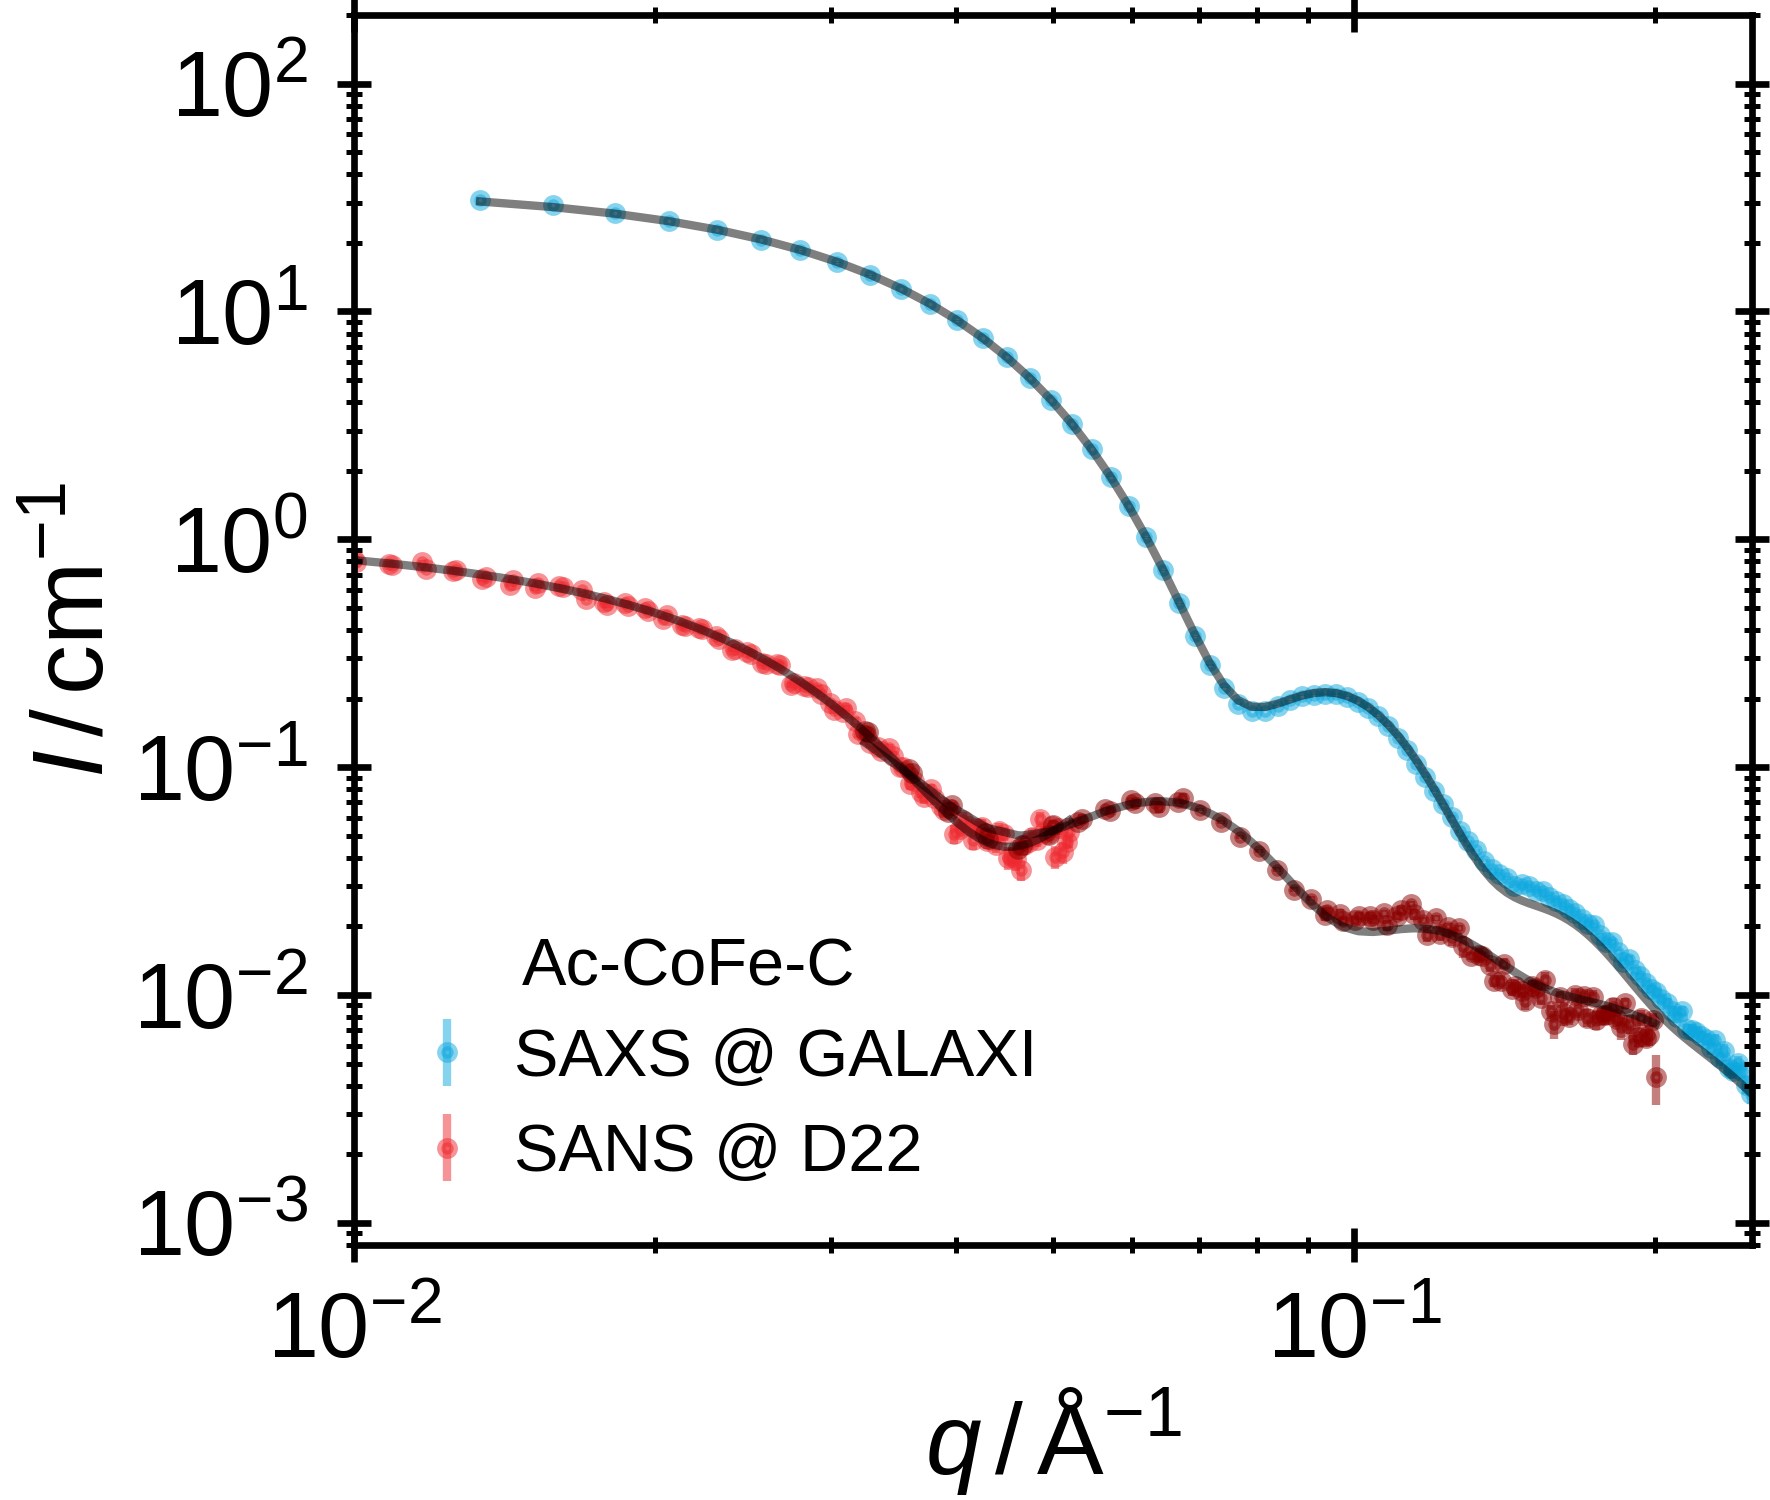
\includegraphics{monolayers_SAS_Ac_CoFe_C_SASFit}
  %     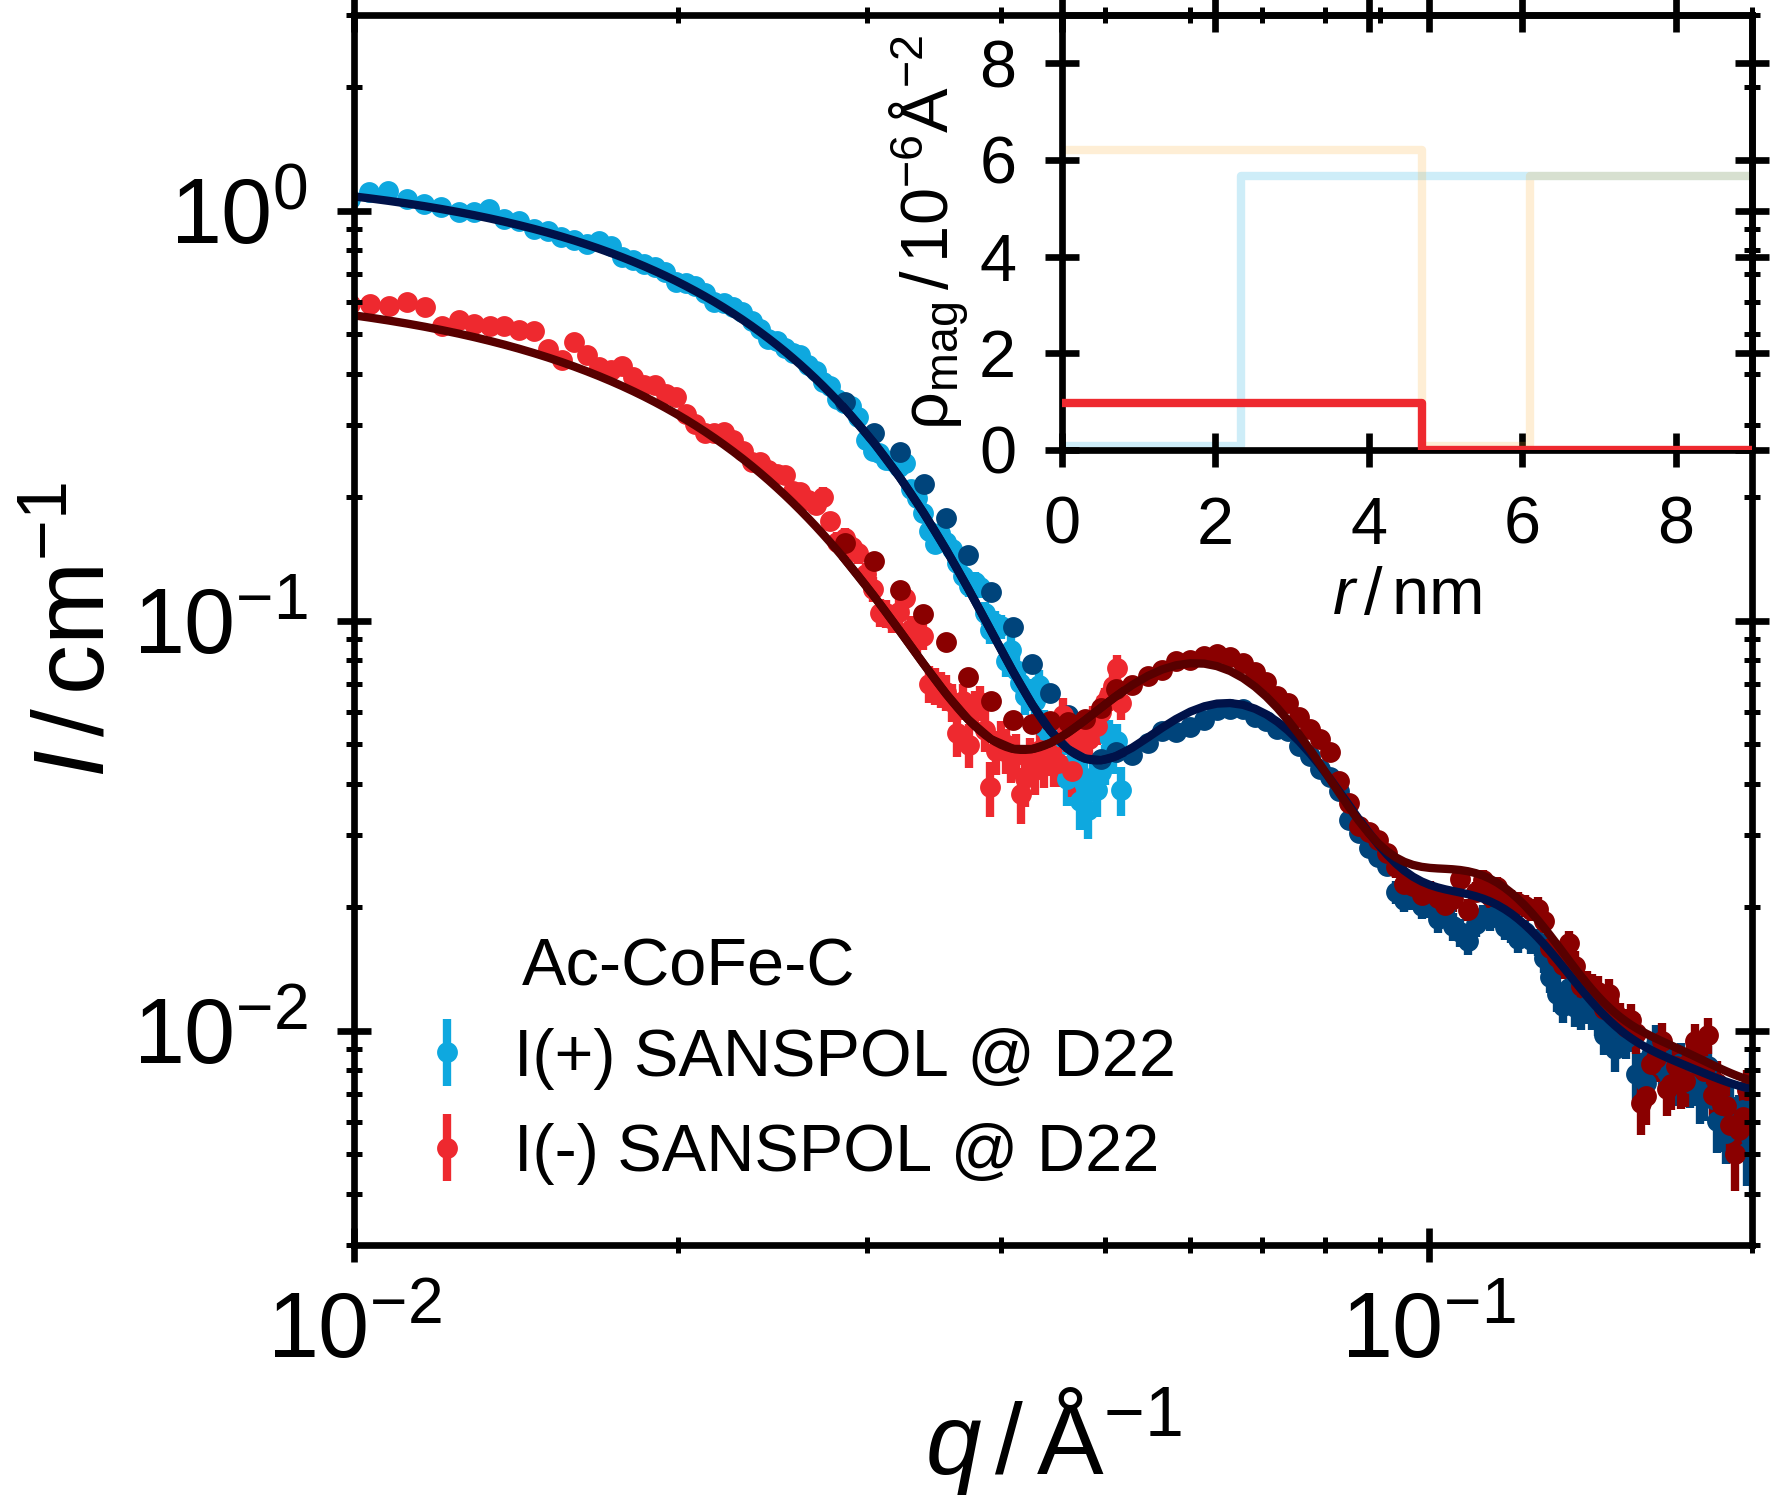
\includegraphics{monolayers_SAS_Ac_CoFe_C_SANSPOLFit}
  %     \caption{\label{fig:monolayers:nanoparticle:sas:AcAcCoFeC}SAXS and SANS measurement of Ol-CoFe-C (upper left) and Ac-CoFe-C (lower left), as well as SANSPOL at $1.2 \unit{T}$ (right). The data is fit to a superball form factor.}
  %   \end{figure}

  %   The surfactant shell thickness are in the range of $1 - 2 \unit{nm}$, which is expected for oleic acid chains.
  %   As the chains mix with the solvent on the way out, it is expected that the average scattering length density of the shell is not exactly that of bulk oleic acid ($7.8 \cdot 10^{-8} \angstrom^{-2}$), but a mixture with the solvent SLD, which correlates with the model thickness and might explain the reduced value in Ac-CoFe-C.
  %   The exact thickness, density and shape of the shell is not of detailed interest for the study of the magnetic properties of the nanocubes and therefore in the scope of this work this rough estimate of the shell is good enough for the discussion.

  %   % SANSPOL <-> VSM at 300K
  %   The magnetic scattering length density is determined from the SANSPOL data, which is used to determine the magnetization of the nanoparticle using \refeq{eq:looselyPackedNP:nanoparticles:SLDtoMagnetization} to $92(3) \unit{kAm^{-1}}$ for Ol-CoFe-C and $145(2) \unit{kAm^{-1}}$ for Ac-CoFe-C.

  %   The fitted model is shown in \reffig{fig:monolayers:nanoparticle:sas:AcAcCoFeC} and the important parameter of interest are given in \reftab{tab:monolayers:nanoparticle:sas} for the following discussion, whereas the full set of model parameters is listed in \refapp{ch:appendix:modelparameters:monolayers:sas_olac_cofe_c}.
  %   \begin{table}[ht]
  %     \centering
  %     \caption{\label{tab:monolayers:nanoparticle:sas}Relevant parameters of the superball fit of the small-angle scattering data of the presented nanocubes, the complete set used to describe the models are found in \refapp{ch:appendix:modelparameters:monolayers:sas_olac_cofe_c}.}
  %     \begin{tabular}{ c | l | l }
  %         & Ol-CoFe-C & Ac-CoFe-C \\
  %       \hline
  %       $R$
  %         & $5.62(2) \unit{nm}$
  %         & $4.69(1) \unit{nm}$\\
  %       $\sigma_R$
  %         & $9.27(8) \,\%$
  %         & $11.9(1) \,\%$\\
  %       $D$
  %         & $1.63(1) \unit{nm}$
  %         & $1.16(4) \unit{nm}$\\
  %       $p$
  %         & $1.54(3) \unit{nm}$
  %         & $2.66(9) \unit{nm}$\\
  %       $\rho_\mathrm{mag}^\mathrm{sans}$
  %         & $0.268(8) \cdot 10^{-6} \angstrom^{-2}$
  %         & $0.423(7) \cdot 10^{-6} \angstrom^{-2}$\\
  %       \hline
  %       $V_p$
  %         & $1030(10) \unit{nm^3}$
  %         & $726(5) \unit{nm}$\\
  %       $M^\mathrm{sans}$
  %         & $92(3) \unit{kAm^{-1}}$
  %         & $145(2) \unit{kAm^{-1}}$\\
  %       \hline
  %     \end{tabular}
  %   \end{table}
  %   The superball model result confirms the qualitative observation that the Ol-CoFe-C nanoparticles have a smaller size distribution than the Ac-CoFe-C cubes.
  %   Where the specimen size used to determine size and size distributions in TEM leave the option for a biased result due to possibly missed counting fractions of the dispersion by only measuring a small selected amount of nanoparticles, the large number of particles scanned in the small-angle scattering experiments reveals without bias the average particle size and variation.
  %   Furthermore, the model gives that on average Ol-CoFe-C has a higher degree of roundness on the corners, visible from the smaller $p$ parameter in comparison to Ac-CoFe-C.
  %   To see this in imaging experiments, high resolution transmission electron microscopy (HR-TEM) experiments are necessary.
  %   A study comparing the effectiveness of the superball model in comparison to HR-TEM can be found in \refapp{app:structureCoFe2O4Nanocubes} for three particle batches synthesized similar to Ac-CoFe-C (with a lower heating rate and varied cobalt content, but otherwise same synthesis parameters).

  % \paragraphNewLine{Impact of Form Factor on Magnetization Density}

  %   It's worthwhile to study the impact of the chosen shape model of the nanoparticle on the result of the magnetic scattering density.
  %   For this purpose, the simpler models of a perfect sphere and cube are fit additionally to the data of Ac-CoFe-C.
  %   These model provide a good reference point for the parameter values and as the models have one less parameter, they are additionally less prone to systematic errors in the fitting routine due to parameter correlations.
  %   The result of the cubic and spherical fit are shown in \reffig{fig:monolayers:nanoparticle:sas:SphereCubeFit} with the relevant parameters listed in \reftab{tab:monolayers:nanoparticle:sasSphereCubeFit}.

  %   \begin{table}[ht]
  %     \centering
  %     \caption{\label{tab:monolayers:nanoparticle:sasSphereCubeFit}Relevant parameters of the sphere and cube fit to the small-angle scattering data of Ac-CoFe-C, the complete set of parameters is found in \refapp{ch:appendix:modelparameters:monolayers:sas_olac_cofe_c}.}
  %     \begin{tabular}{ c | l | l }
  %         & Sphere & Cube \\
  %       \hline
  %       $R, \, a$
  %         & $5.56(2) \unit{nm}$
  %         & $9.01(2) \unit{nm}$\\
  %       $\sigma_R, \, \sigma_a$
  %         & $13.0(3) \,\%$
  %         & $10.7(2) \,\%$\\
  %       $D$
  %         & $1.46(4) \unit{nm}$
  %         & $1.03(4) \unit{nm}$\\
  %       $\rho_\mathrm{mag}^\mathrm{sans}$
  %         & $0.502(8) \cdot 10^{-6} \angstrom^{-2}$
  %         & $0.429(7) \cdot 10^{-6} \angstrom^{-2}$\\
  %       \hline
  %       $V_p$
  %         & $720(4) \unit{nm^{3}}$
  %         & $731(3) \unit{nm^{3}}$\\
  %       $M^\mathrm{sans}$
  %         & $172(3) \unit{kAm^{-1}}$
  %         & $147(2) \unit{kAm^{-1}}$\\
  %       \hline
  %     \end{tabular}
  %   \end{table}

  %   It's clearly visible by looking at the SAXS data that the spherical model underestimates the intensity of the first order peak, while the cube model overestimates it, whereas the superball was able to adjust in between.
  %   The determined particle volume varies only weakly from the specific choice of the model and therefore the model has only a minor effect on the rescaling procedure that is applied to the vibrating sample magnetometry data.
  %   From SANSPOL, it is visible that parameters such as the shell thickness, particle magnetization, as well as the particle concentration (listed in complete parameter set in \refapp{ch:appendix:modelparameters:monolayers:sas_olac_cofe_c}), are stronger affected by the choice of model in the fitting process.
  %   This becomes especially visible in the observation that the cube model estimates a smaller shell thickness and magnetization, whereas the sphere model suggests values that are a magnitude of $30 - 50 \unit{\%}$ higher.

  %   \begin{figure}[tb]
  %     \centering
  %     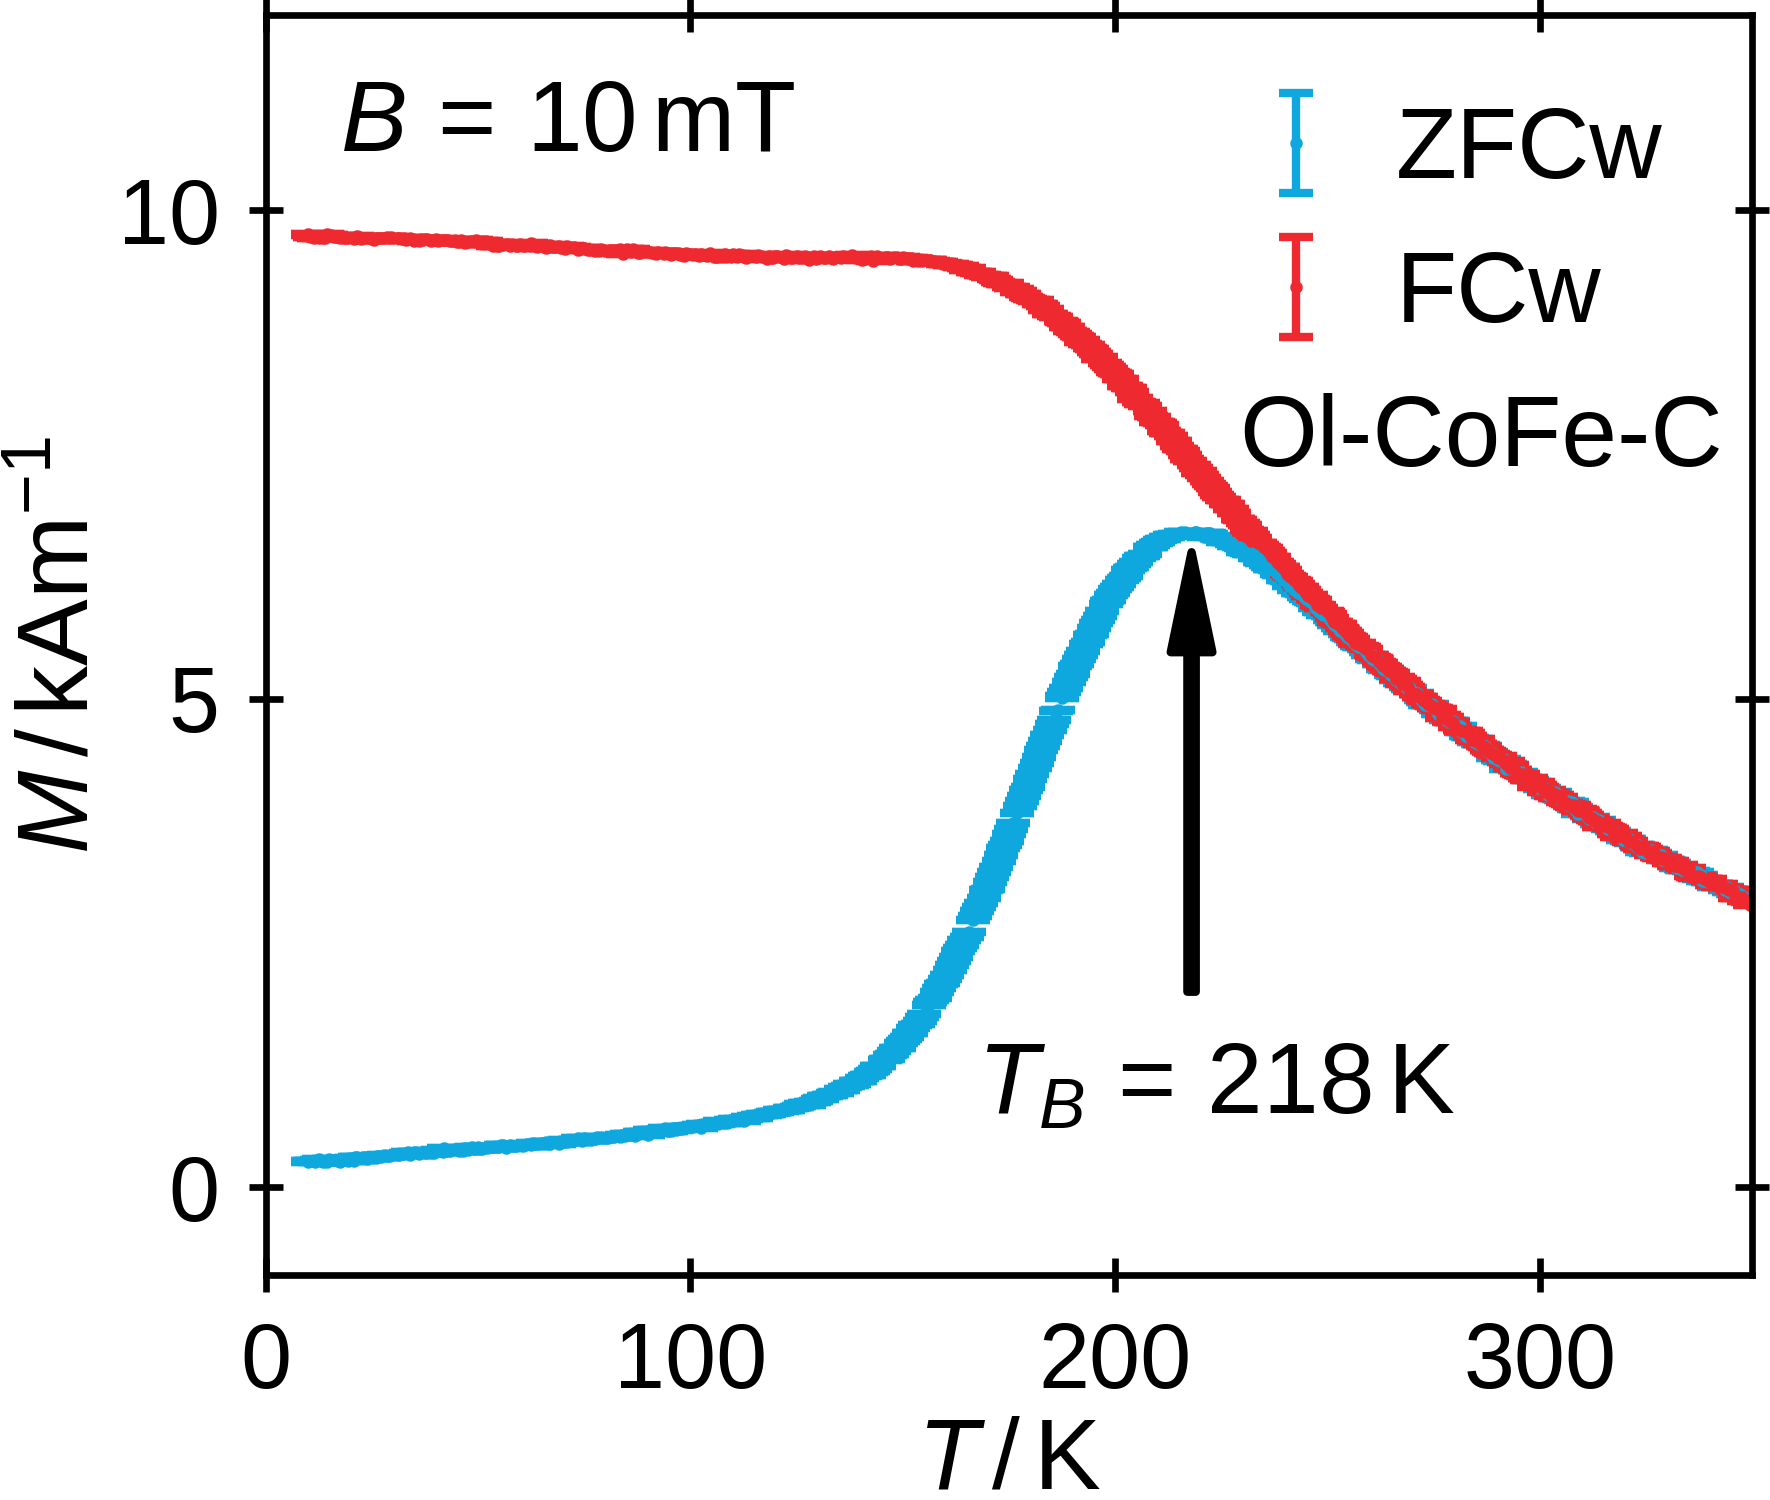
\includegraphics{monolayer_PPMS_ZFC_FC_ML_Ol_CoFe_C}
  %     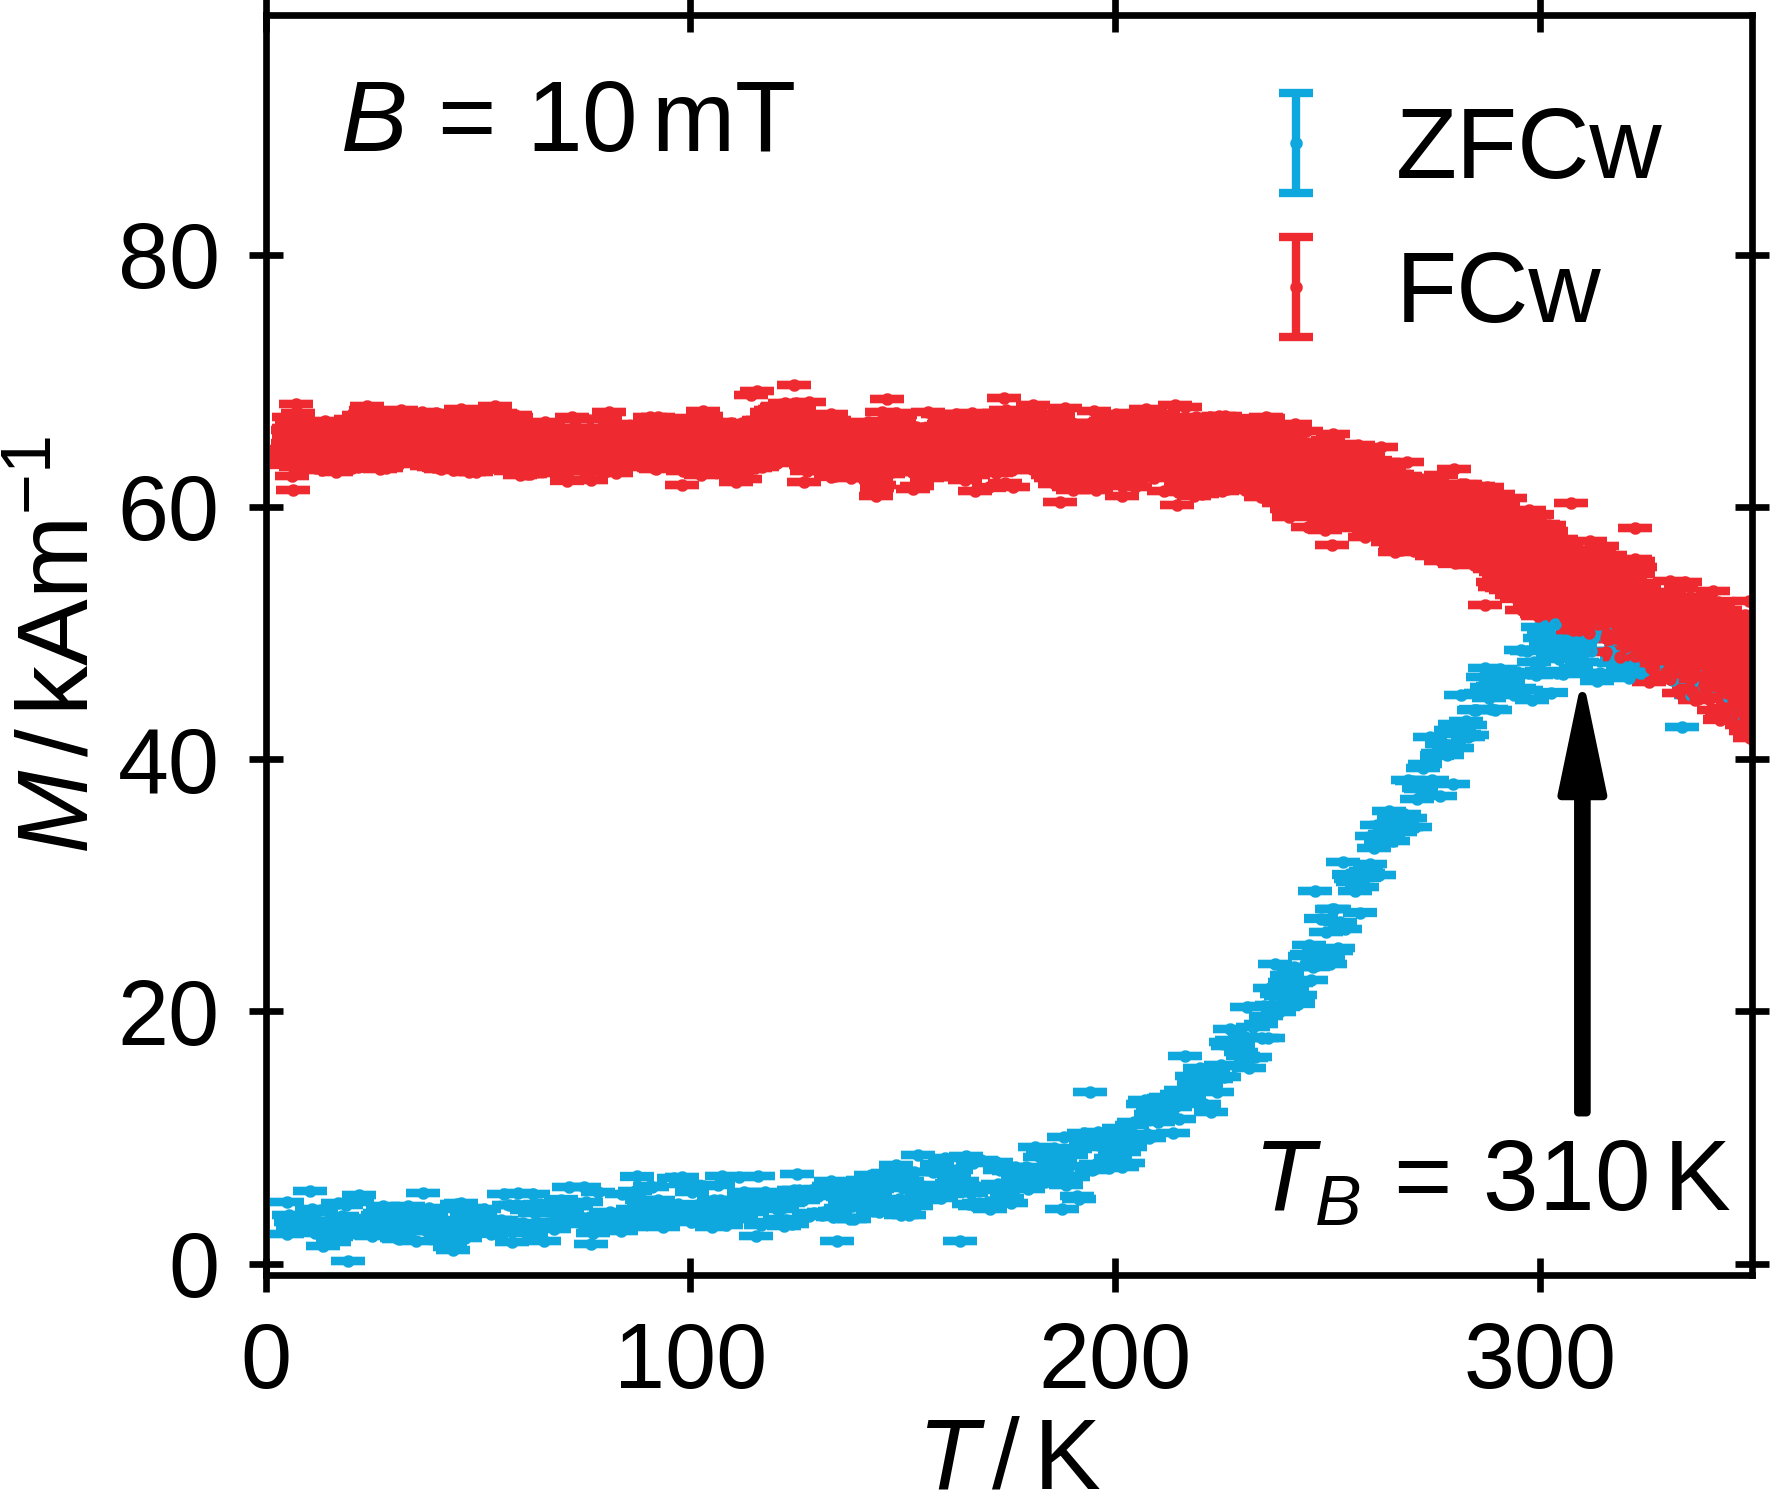
\includegraphics{monolayer_PPMS_ZFC_FC_ML_Ac_CoFe_C}
  %     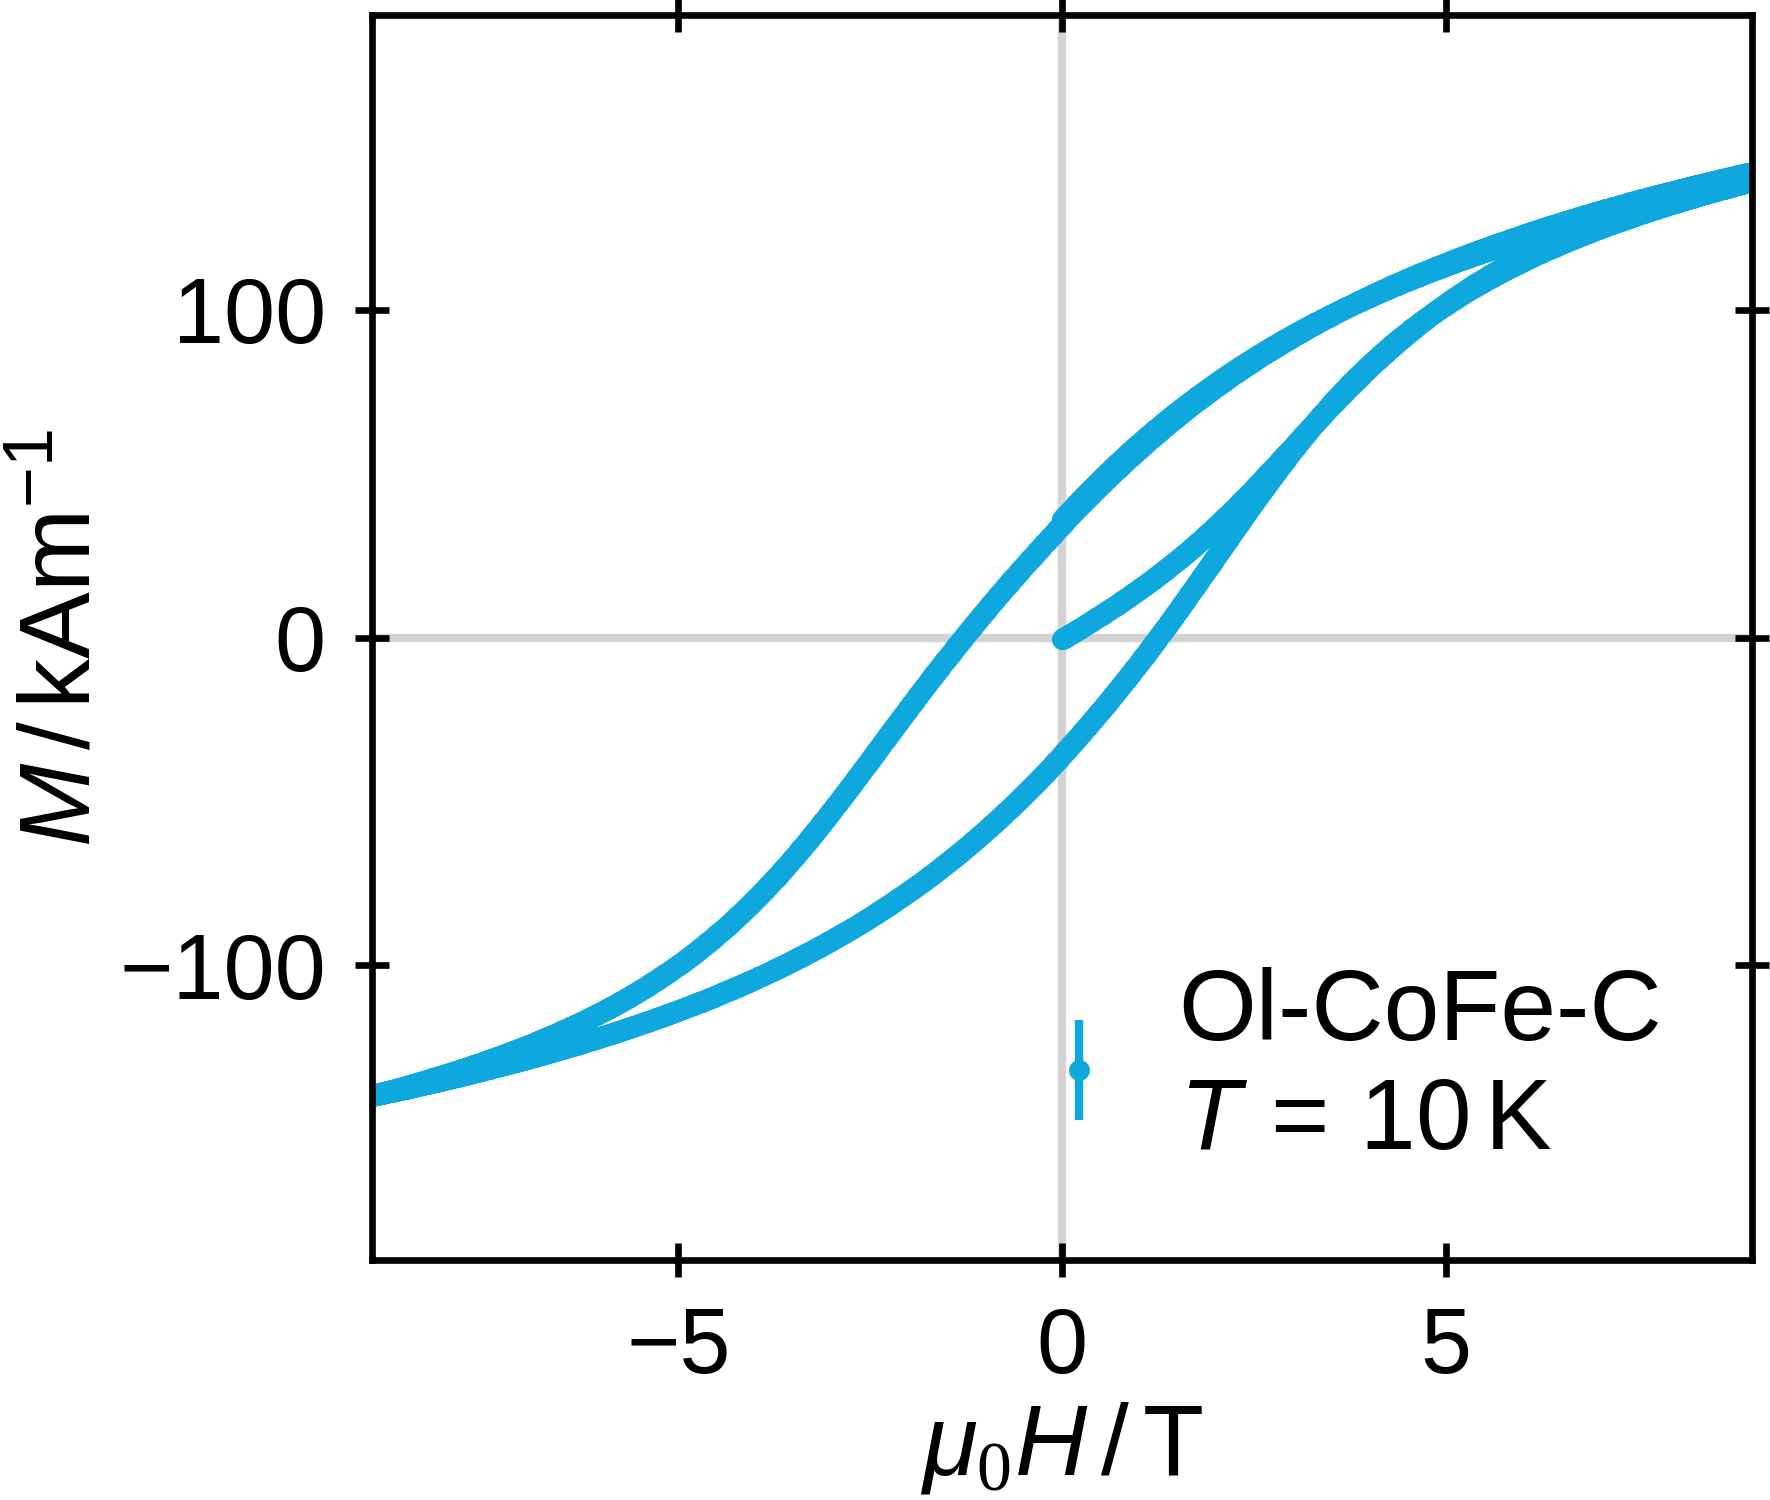
\includegraphics{monolayer_VSM_10K_Ol_CoFe_C}
  %     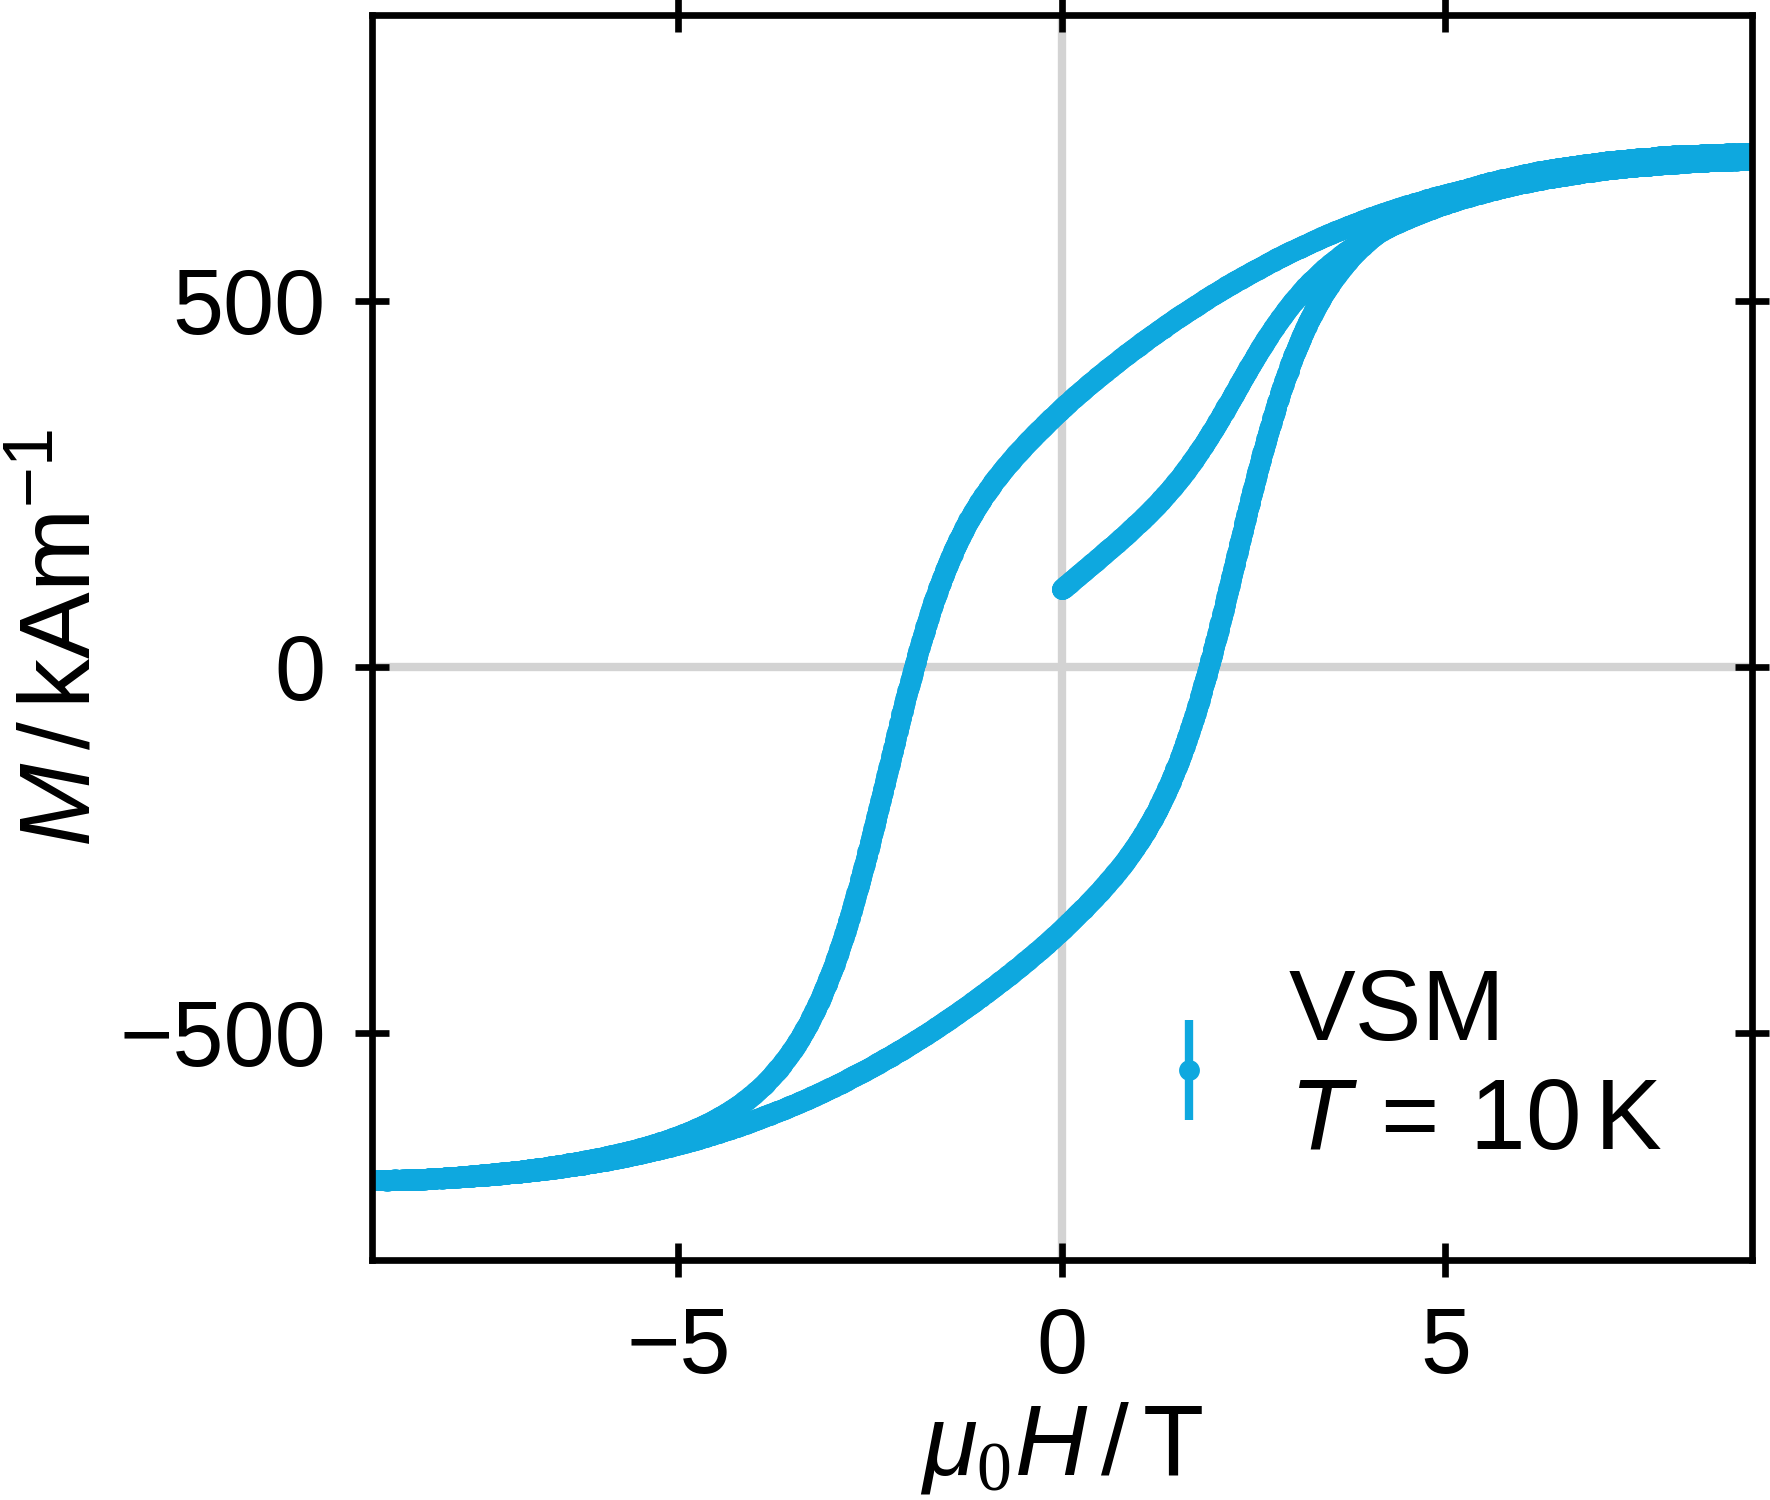
\includegraphics{monolayer_VSM_10K_Ac_CoFe_C}
  %     \caption{\label{fig:monolaye rs:nanoparticle:vsm10K}Low temperature hysteresis measurement of frozen Ol-CoFe-C (left) and Ac-CoFe-C (right) using the same samples as in \reffig{fig:monolayers:nanoparticle:vsm}.}
  %   \end{figure}

  %   \begin{figure}[tb]
  %     \centering
  %     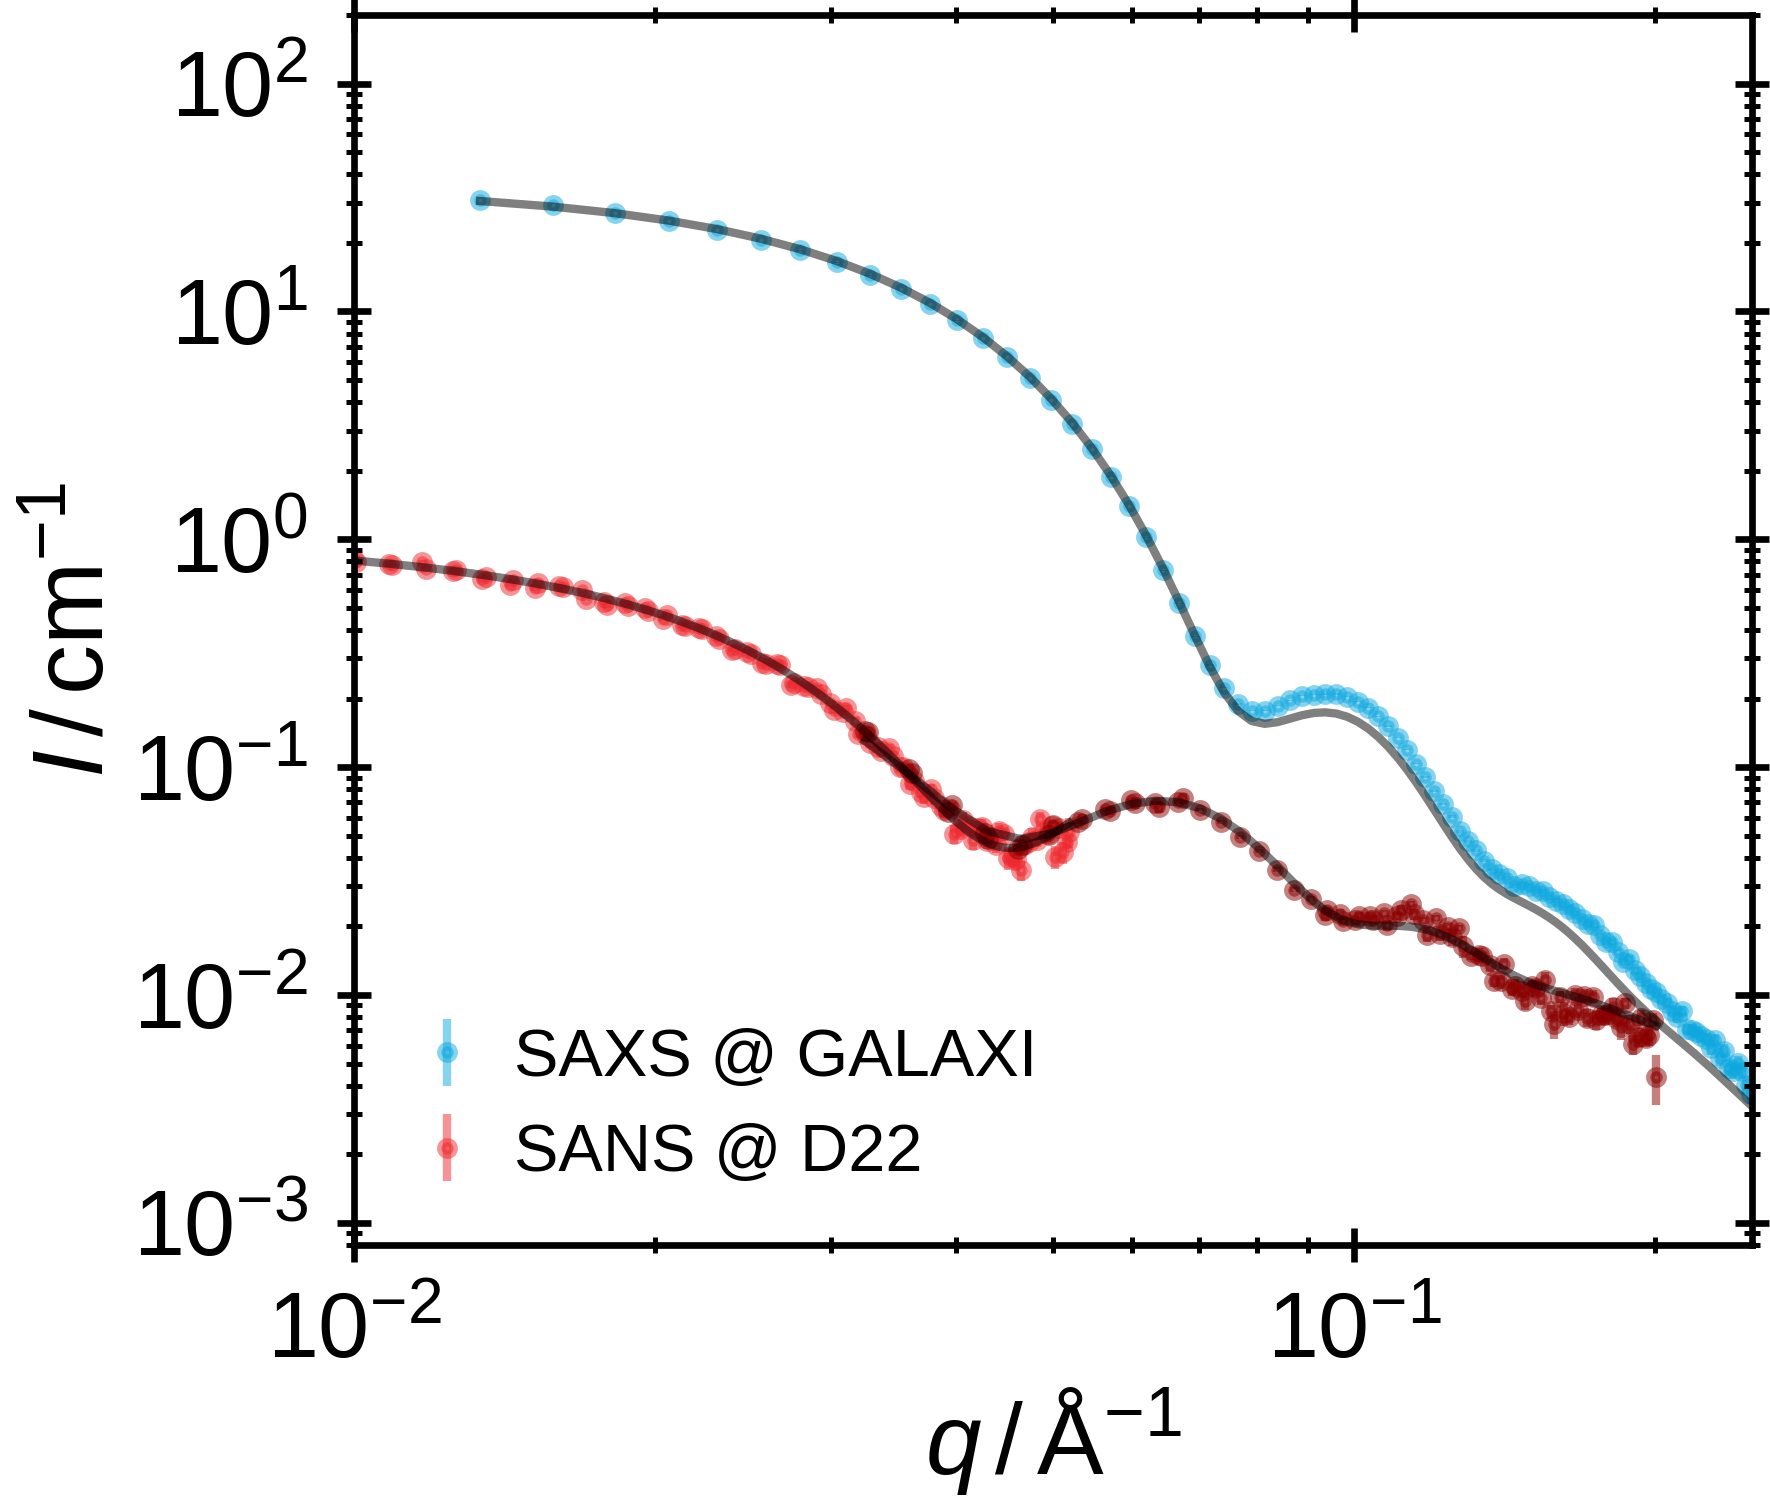
\includegraphics{monolayers_SAS_Ac_CoFe_C_SASSphereModelFit}
  %     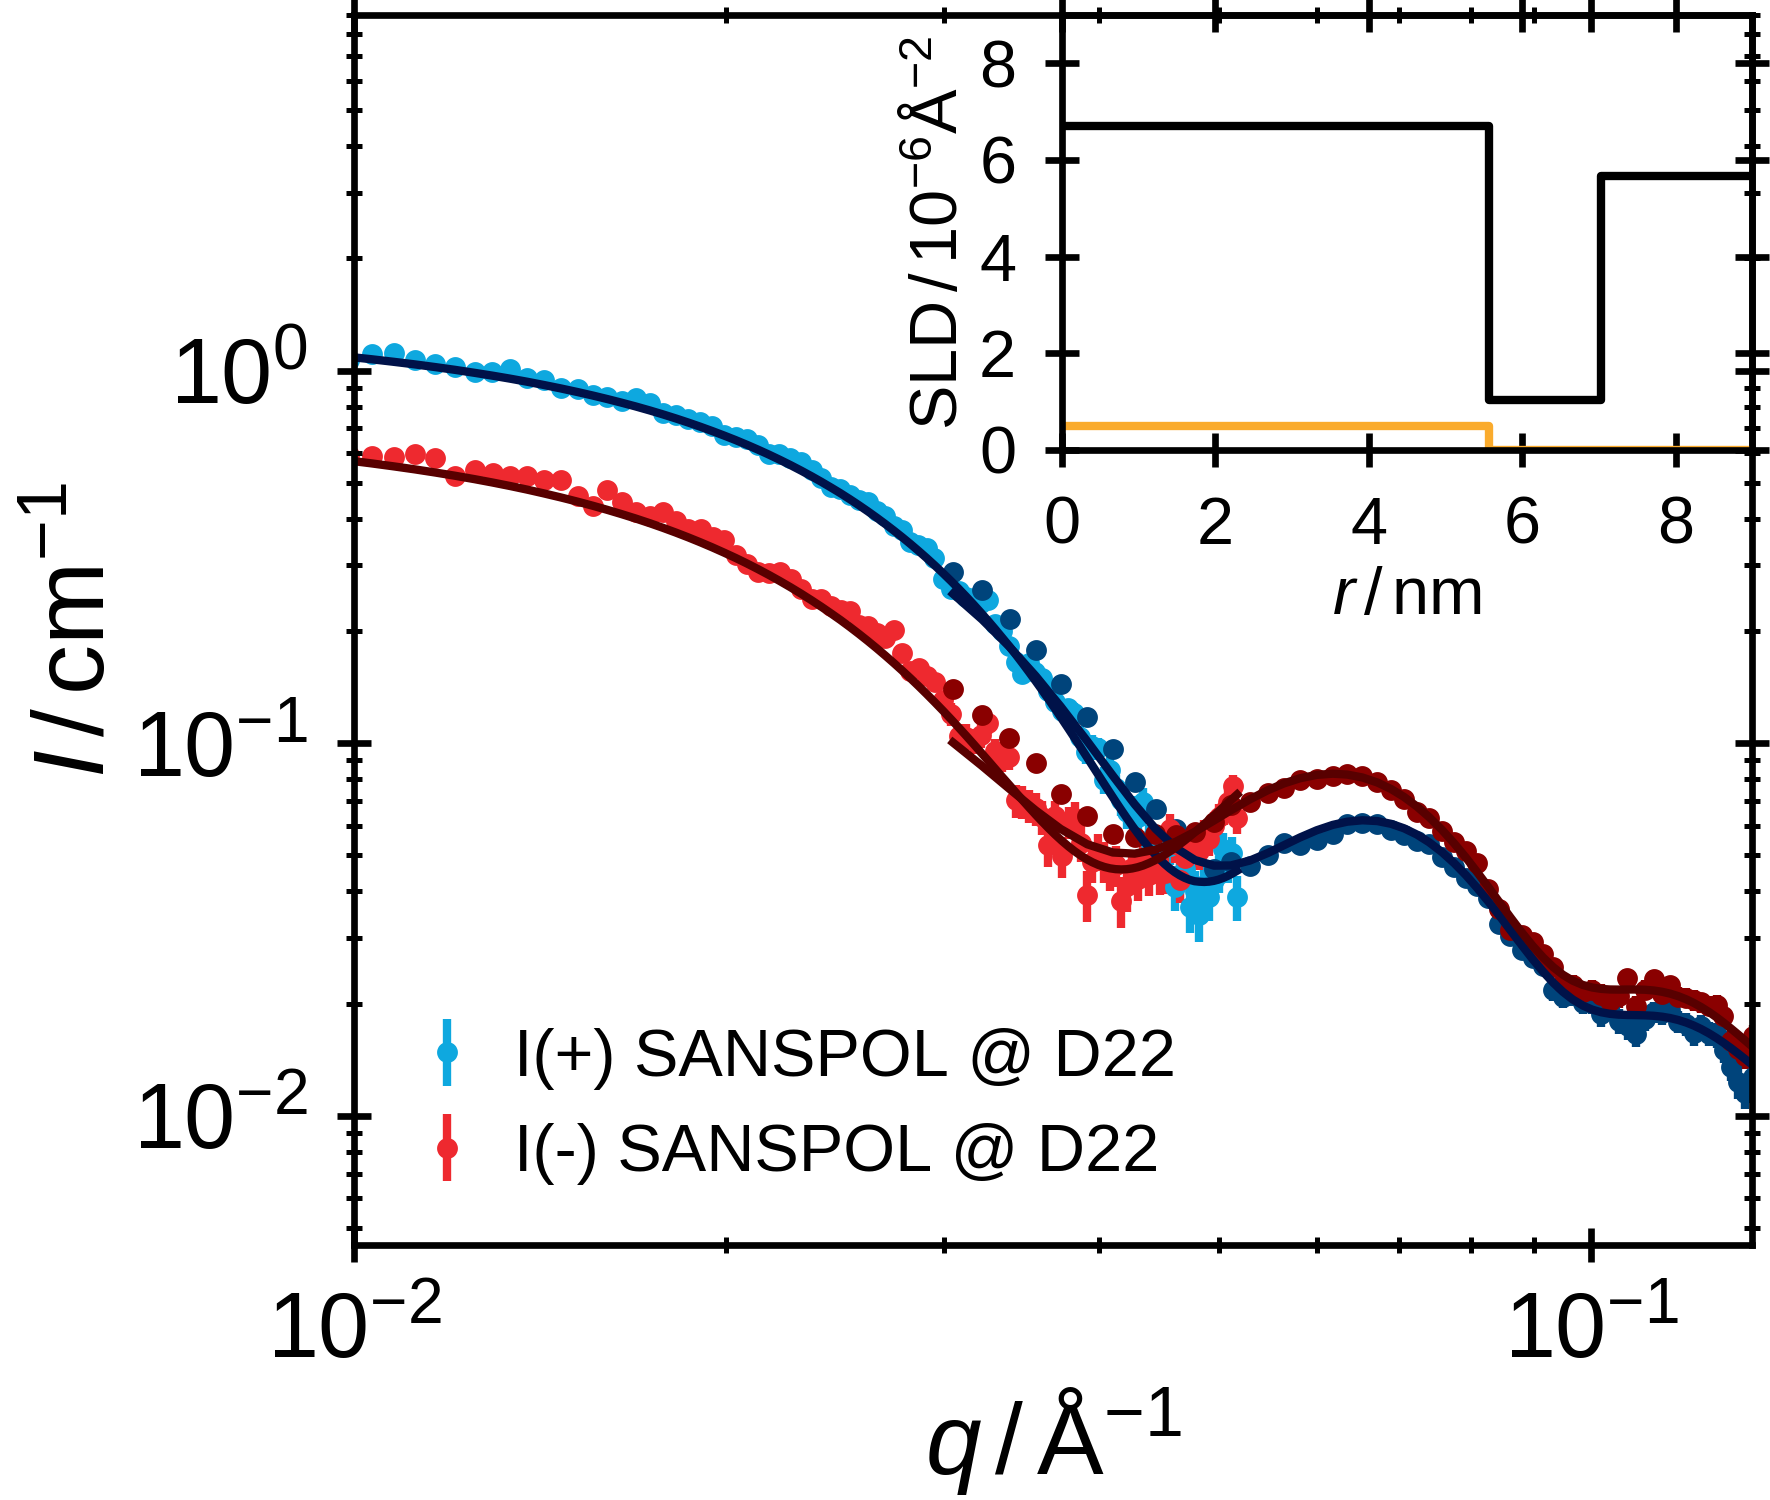
\includegraphics{monolayers_SAS_Ac_CoFe_C_SANSPOLSphereModelFit}
  %     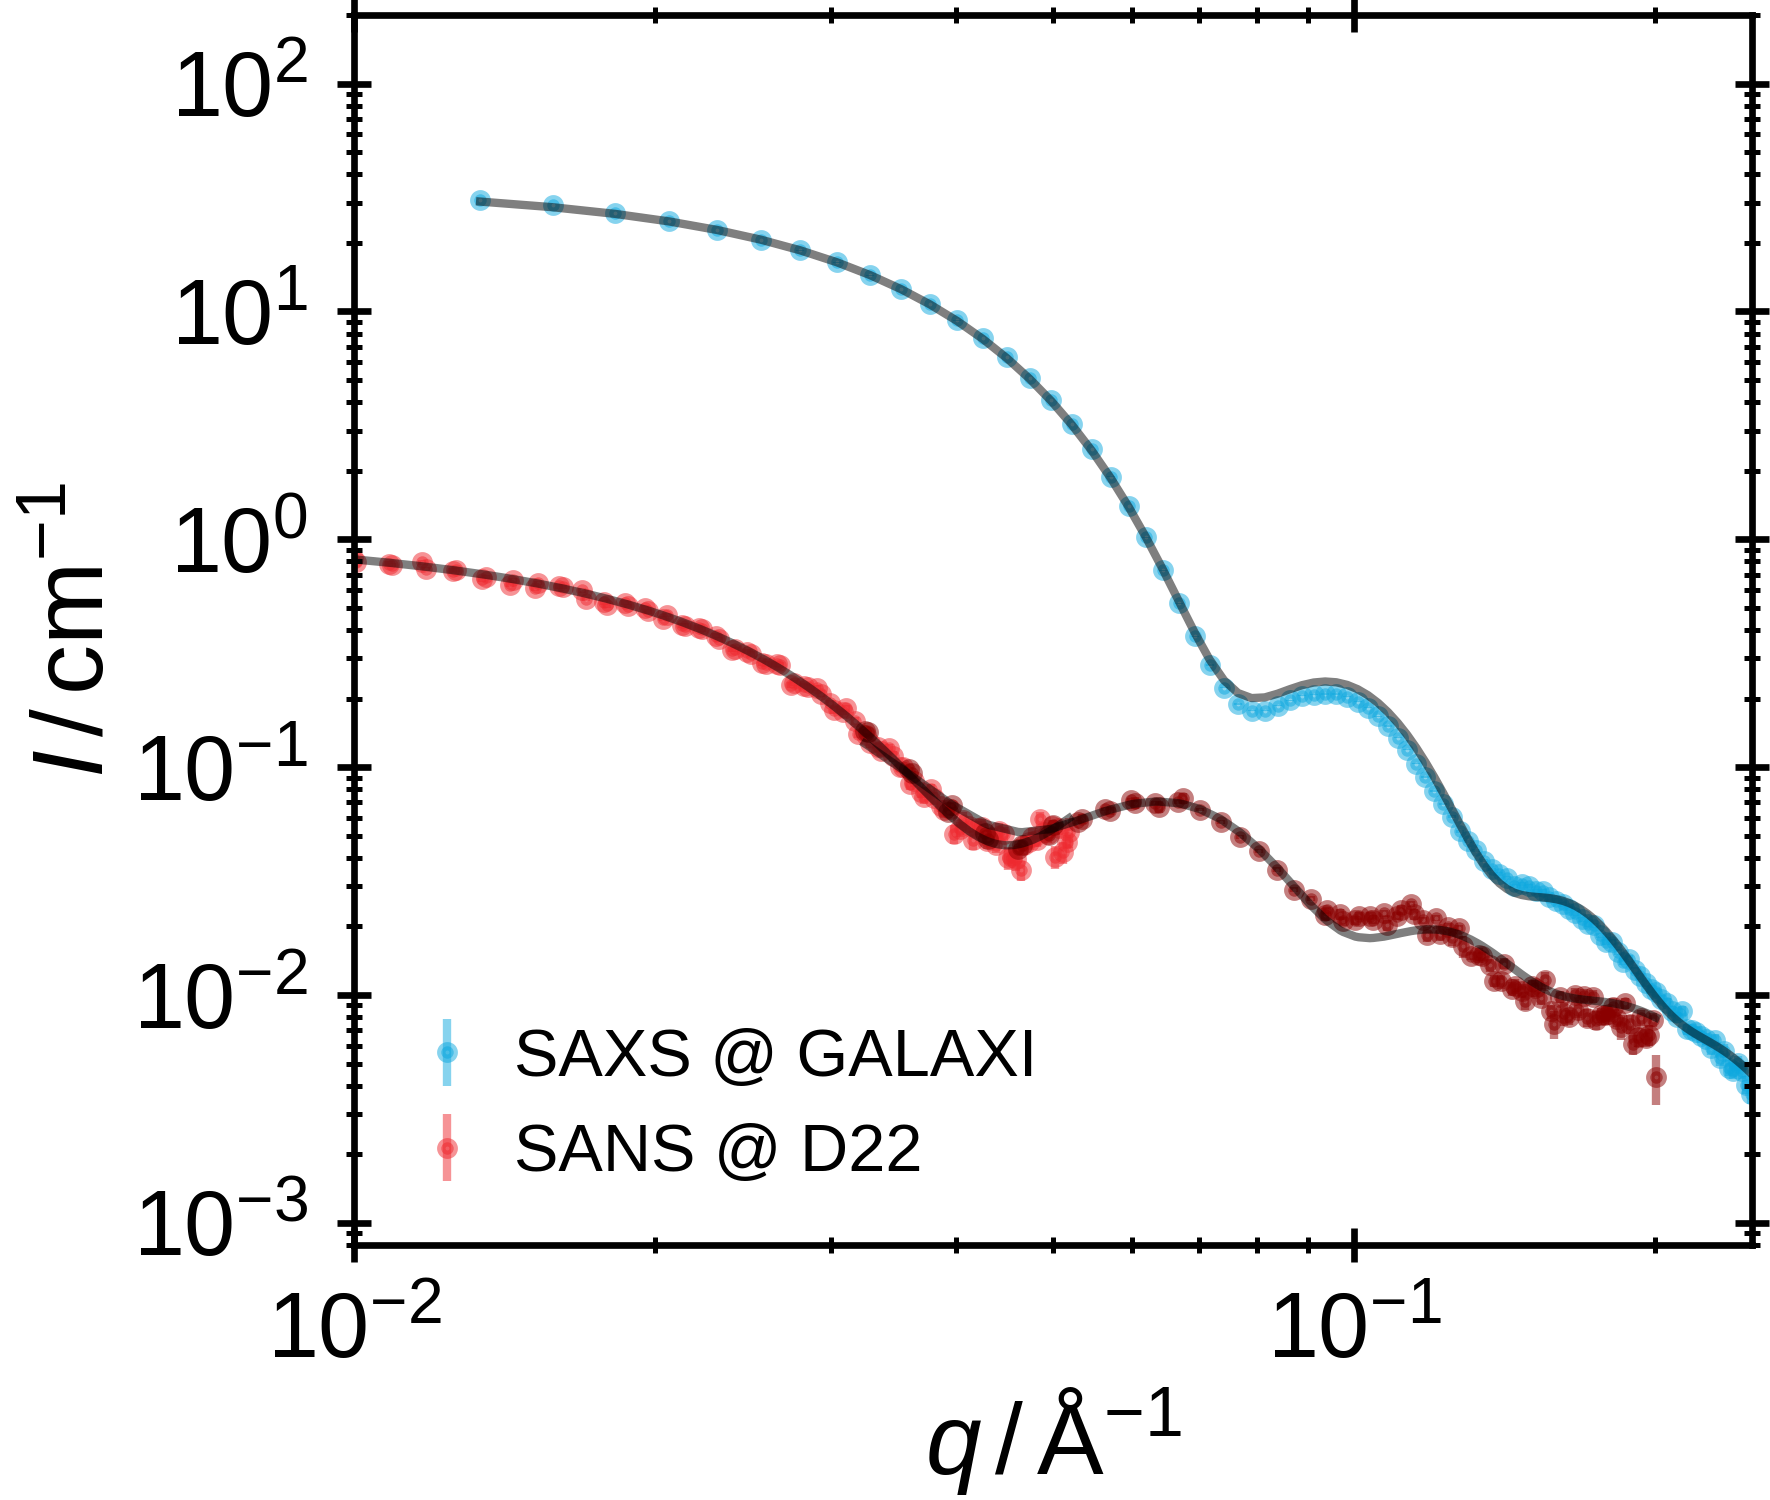
\includegraphics{monolayers_SAS_Ac_CoFe_C_SASCubeModelFit}
  %     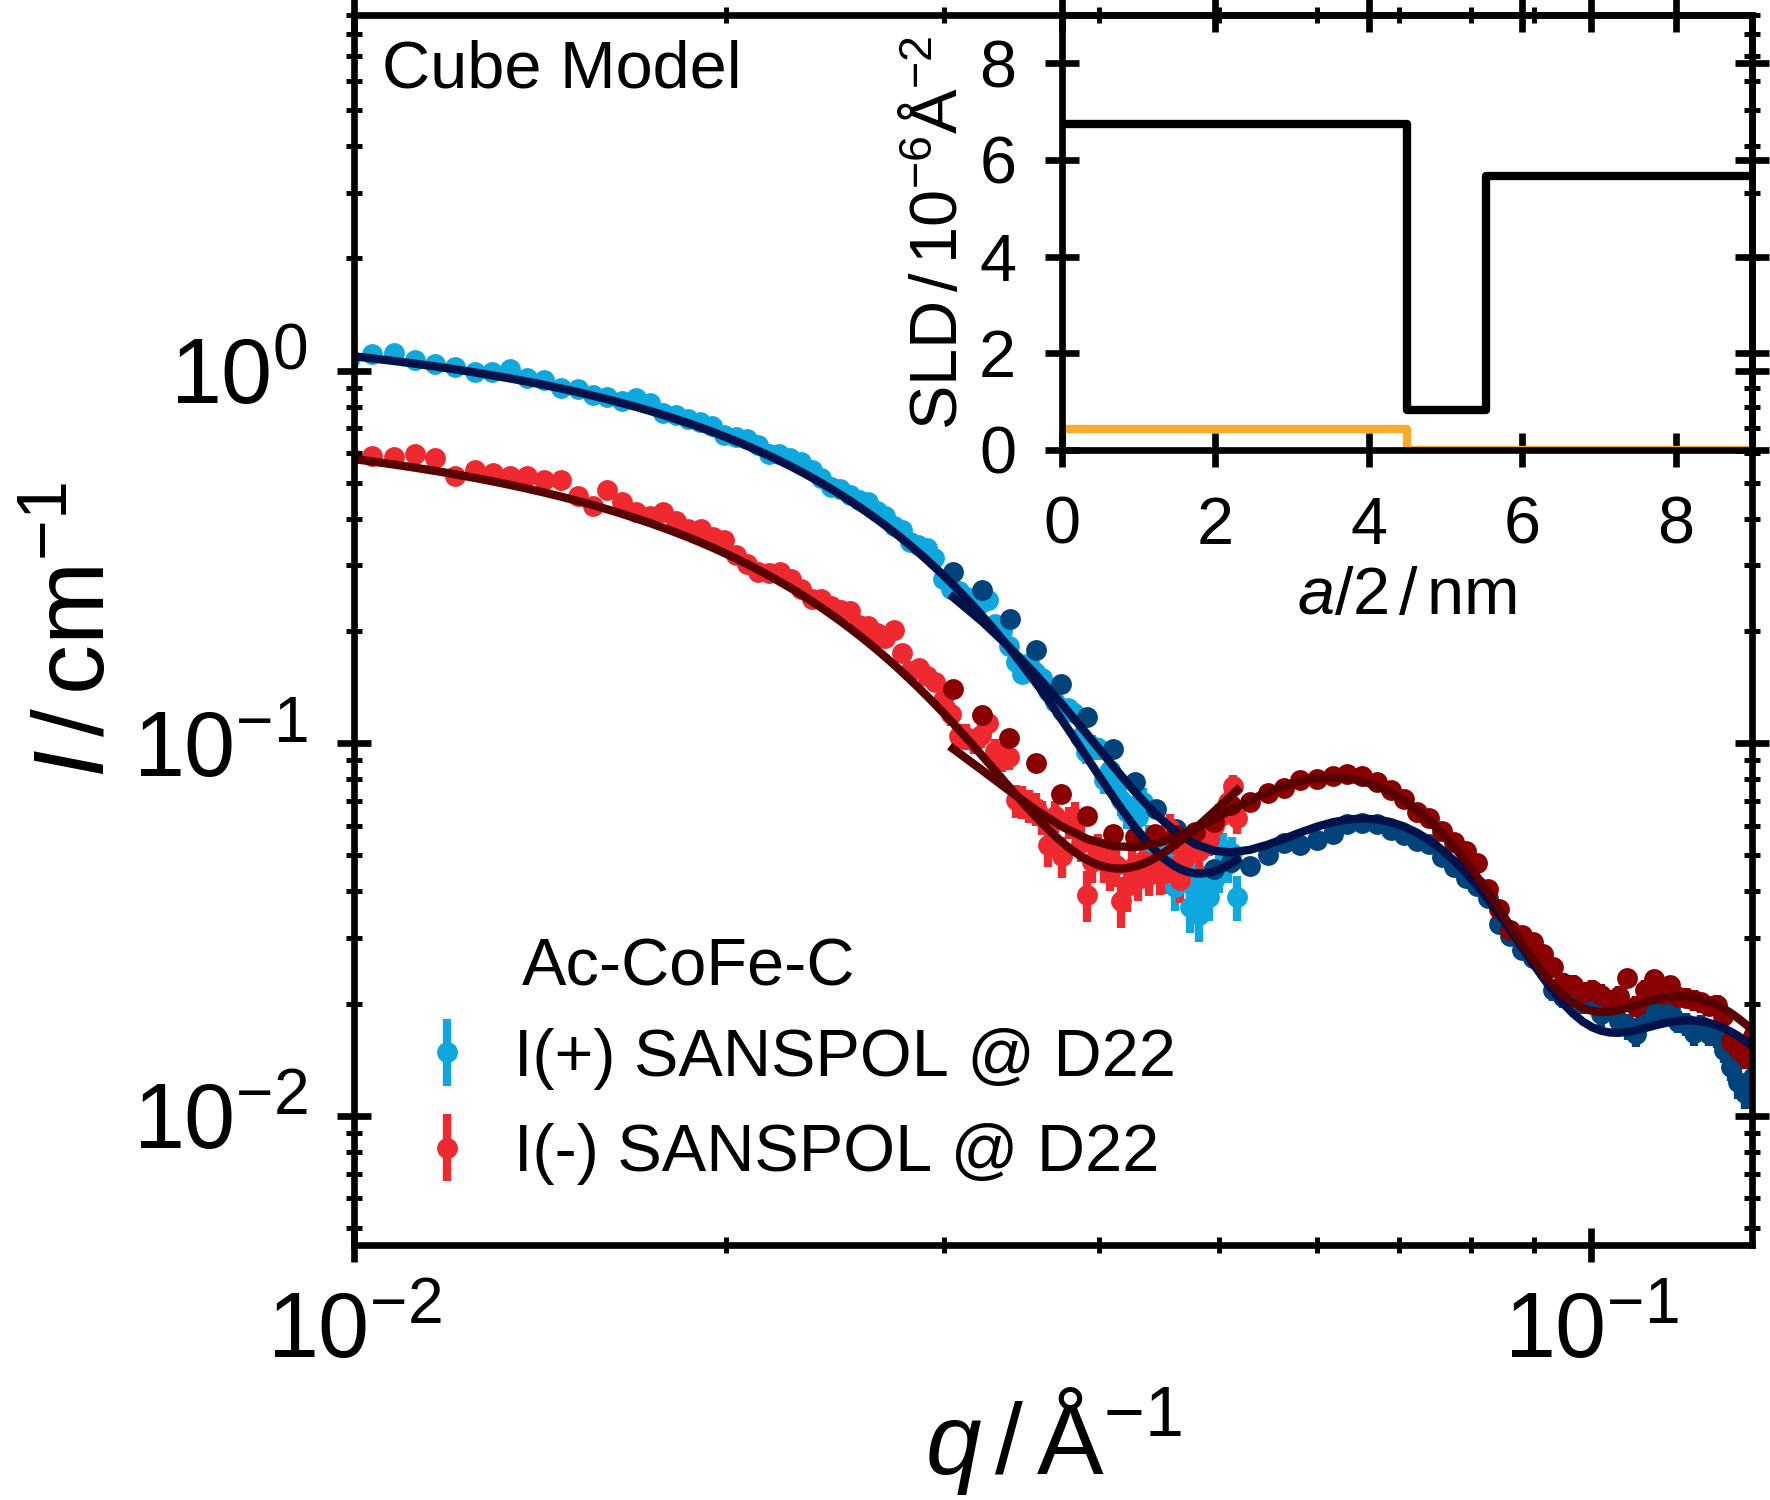
\includegraphics{monolayers_SAS_Ac_CoFe_C_SANSPOLCubeModelFit}
  %     \caption{\label{fig:monolayers:nanoparticle:sas:SphereCubeFit}Best sphere (upper) and cube model (lower) fit to the same SAS data of Ac-CoFe-C fitted in \reffig{fig:monolayers:nanoparticle:sas:AcAcCoFeC}. The left images show the fit of the nuclear structure for the two models, and the right the determination of the magnetic structure.}
  %   \end{figure}
\end{document}